%% 
%%  An UIT Edition example
%% 
%%  Example 04-27-26 on page 146.
%% 
%%  Copyright (C) 2012 Vo\ss 
%% 
%%  It may be distributed and/or modified under the conditions
%%  of the LaTeX Project Public License, either version 1.3
%%  of this license or (at your option) any later version.
%% 
%%  See http://www.latex-project.org/lppl.txt for details.
%% 

% Show page(s) 1,2,3

%% ==== 
\PassOptionsToClass{}{beamer}
\documentclass[serif, aspectratio=169]{beamer}
\usepackage[utf8]{inputenc}

%\StartShownPreambleCommands
\usepackage{amsmath,esint}
\usepackage[british]{babel}
\usetheme{Warsaw}
\usecolortheme{rose}

%\usetheme{metropolis}
%\usepackage{appendixnumberbeamer}

%\StopShownPreambleCommands
\usepackage{pgfplots}
\usepackage{ mathrsfs }
\usepackage{caption}
\usepackage{ragged2e}

\usepackage{gensymb}
\usepackage{color}
\usepackage{url}
\usetikzlibrary{shapes,backgrounds,calc}

\usepackage{tkz-euclide}
\usetkzobj{all}
\usepackage{tkz-fct}  
\usetikzlibrary{calc}
\usepackage{tikz,calc}

\usepackage[ruled]{algorithm2e}
\usepackage{tikz}
\usetikzlibrary{arrows.meta}
\usepackage{animate}
\DeclareMathOperator*{\minimize}{minimize}

\addtobeamertemplate{navigation symbols}{}{%
    \usebeamerfont{footline}%
    \usebeamercolor[fg]{footline}%
    \hspace{1em}%
    \insertframenumber/\inserttotalframenumber
    }

    \renewcommand{\thealgocf}{}

    \usepackage[labelformat=empty]{caption}
    \makeatletter
    \newcommand\titlegraphicii[1]{\def\inserttitlegraphicii{#1}}
    \titlegraphicii{}
    \setbeamertemplate{title page}
    {
    \vspace{0.3in}
    \vbox{}
   %{\usebeamercolor[fg]{titlegraphic}\inserttitlegraphic\hfill\inserttitlegraphicii\par}
   \begin{centering}
   \begin{beamercolorbox}[sep=8pt,center]{title}
      \usebeamerfont{title}\inserttitle\par%
      \ifx\insertsubtitle\@empty%
      \else%
        \vskip0.25em%
        {\usebeamerfont{subtitle}\usebeamercolor[fg]{subtitle}\insertsubtitle\par}%
      \fi%     
    \end{beamercolorbox}%
    \vskip1em\par
    \begin{beamercolorbox}[sep=8pt,center]{date}
    \usebeamerfont{date}\insertdate
    \end{beamercolorbox}%\vskip0.5em
    \begin{beamercolorbox}[sep=8pt,center]{author}
    \usebeamerfont{author}\insertauthor
    \end{beamercolorbox}
    \begin{beamercolorbox}[sep=8pt,center]{institute}
    \usebeamerfont{institute}\insertinstitute
    \end{beamercolorbox}
    \end{centering}
  %\vfill
  }
  \makeatother
%\author{Anirban Laha and Preksha Nema \\\vspace{0.2in} Presented By: Mitesh M. Khapra}
\author{Mitesh M. Khapra}
\title{CS7015 (Deep Learning) : Lecture 2}
\subtitle{McCulloch Pitts Neuron, Thresholding Logic, Perceptrons, Perceptron Learning Algorithm and Convergence, Multilayer Perceptrons (MLPs), Representation Power of MLPs}
\institute{Department of Computer Science and Engineering\\ Indian Institute of Technology Madras}
\titlegraphic{
\includegraphics[height=1cm,width=2cm]{images/iitm_logo.png}}
\date{}
%\titlegraphicii{\includegraphics[height=1cm,width=2cm]{logo2}}

\newcommand\myheading[1]{%
\par\bigskip
{\Large\bfseries#1}\par\smallskip}


\begin{document}


\renewcommand{\thefootnote}{$\star$} 

\tikzset{
o/.style={
shorten >=#1,
decoration={
markings,
mark={
at position 1
with {
\draw circle [radius=#1];
}
}
},
postaction=decorate
},
o/.default=2pt
}

\newcommand\derivative[5]{%
\tkzDefPointByFct[draw](#1) \tkzGetPoint{start}
\tkzDefPointByFct[draw](#2) \tkzGetPoint{end}
\draw[thin,|-|,yshift=-3pt] (start) -- node[black,fill=white,#5] {#3}(start-|end);  
\draw[thin,|-|,xshift=3pt] (start-|end) -- node[black,fill=white,right] {#4}(end); 
  %\draw[thin] (start) --(end); 
  }

\tikzstyle{input_neuron}=[circle,draw=red!50,fill=orange!10,thick,minimum size=1mm]
\tikzstyle{hidden_neuron}=[circle,draw=blue!50,fill=blue!10,thick,minimum size=10mm]
\tikzstyle{output_neuron}=[circle,draw=green!50,fill=green!20,thick,minimum size=4mm]

\tikzstyle{input}=[circle,draw=black!50,fill=black!20,thick,minimum size=.2mm]
  \maketitle

  \begin{frame}
    \myheading{Module 2.1: Biological Neurons}
  \end{frame}
  \begin{frame}

  \begin{columns}

  \column{0.5\textwidth}
  \begin{overlayarea}{\textwidth}{\textheight}

  \tikzstyle{input_neuron}=[circle,draw=red!50,fill=orange!10,thick,minimum size=1mm]
  \tikzstyle{hidden_neuron}=[circle,draw=blue!50,fill=blue!10,thick,minimum size=10mm]
  \tikzstyle{output_neuron}=[circle,draw=green!50,fill=green!20,thick,minimum size=4mm]

  \tikzstyle{input}=[circle,draw=black!50,fill=black!20,thick,minimum size=.2mm]

  \begin{figure}
  \centering
  \begin{tikzpicture}

  \node (input0) at (9,-0.1)  {$x_{1}$};
  \node (input1) at (10,-0.1)  {$x_{2}$};
  \node (input2) at (11,-0.1)  {$x_{3}$};
  \node [hidden_neuron] (neuron1) at (10,2)  {$\sigma$};


  \node (output0)  at (10,3.5) {$y$};

  \draw [->] (input0) -- (neuron1);
  \draw [->] (input1) -- (neuron1);
  \draw [->] (input2) -- (neuron1);

  \draw [->] (neuron1) -- (output0);

  \node (formula)[scale=.8] at (9.1,0.6) {$w_{1}$};
  \node (formula)[scale=.8] at (9.8,0.6) {$w_{2}$};
  \node (formula)[scale=.8] at (10.4,0.6) {$w_{3}$};
  \end{tikzpicture}
  \caption{Artificial Neuron}
  \end{figure}
  \end{overlayarea}

  \column{0.5\textwidth}
  \begin{overlayarea}{\textwidth}{\textheight}

  \begin{itemize}
    \justifying
    \item<1-> The most fundamental unit of a deep neural network is called an \textit{artificial neuron}
    \item<2-> Why is it called a neuron ? Where does the inspiration come from ?
    \item<3-> The inspiration comes from biology (more specifically, from the \textit{brain})
    \item<4-> \textit{biological neurons = neural cells = neural processing units}
    \item<5-> We will first see what a biological neuron looks like ...

  \end{itemize}
  \end{overlayarea}
  \end{columns}
  \end{frame}


  \begin{frame}
  \begin{columns}

  \column{0.5\textwidth}
  \begin{overlayarea}{\textwidth}{\textheight}


  \only<1->{
  \begin{figure}
  \centering
  \includegraphics<1>[scale= 0.3]{images/BioNeuron1.png}
  \includegraphics<2>[scale= 0.3]{images/BioNeuron2.png}
  \includegraphics<3>[scale= 0.3]{images/BioNeuron3.png}
  \includegraphics<4>[scale= 0.3]{images/BioNeuron4.png}
  \includegraphics<5>[scale= 0.3]{images/BioNeuron5.png}
  \caption{Biological Neurons$^*$\vspace{0.4in}\footnotetext{$^*$Image adapted from \url{https://cdn.vectorstock.com/i/composite/12,25/neuron-cell-vector-81225.jpg}}}
  \end{figure}
  }
  \end{overlayarea}

  \column{0.5\textwidth}
  \begin{overlayarea}{\textwidth}{\textheight}
  \begin{itemize}\justifying
  \item<2-> \textbf{dendrite:} receives signals from other neurons
  \item<3-> \textbf{synapse:} point of connection to other neurons
  \item<4-> \textbf{soma:} processes the information
  \item<5-> \textbf{axon:} transmits the output of this neuron
\end{itemize}
\end{overlayarea}
\end{columns}
\end{frame}


\begin{frame}
\begin{columns}

\column{0.5\textwidth}
\begin{overlayarea}{\textwidth}{\textheight}


\begin{figure}
\centering
\includegraphics<2>[scale= 0.5]{images/SheldonExample2.png}
\includegraphics<3>[scale= 0.5]{images/SheldonExample3.png}
\includegraphics<4>[scale= 0.5]{images/SheldonExample4.png}
\end{figure}
\end{overlayarea}

\column{0.5\textwidth}
\begin{overlayarea}{\textwidth}{\textheight}
\begin{itemize}\justifying

\item<1-> Let us see a very cartoonish illustration of how a neuron works
\item<2-> Our sense organs interact with the outside world
\item<3-> They relay information to the neurons
\item<4-> The neurons (may) get activated and produces a response (laughter in this case)

\end{itemize}
\end{overlayarea}
\end{columns}
\end{frame}

\begin{frame}
\begin{columns}

\column{0.4\textwidth}
\begin{overlayarea}{\textwidth}{\textheight}

\begin{figure}
\centering
\includegraphics<1-3>[scale= 0.4]{images/BigSheldonExample1.png}
\includegraphics<4>[scale= 0.4]{images/BigSheldonExample2.png}
\includegraphics<5>[scale= 0.4]{images/BigSheldonExample3.png}
\includegraphics<6->[scale= 0.4]{images/BigSheldonExample4.png}
\end{figure}
\end{overlayarea}

\column{0.6\textwidth}
\begin{overlayarea}{\textwidth}{\textheight}
\begin{itemize}\justifying

\item<1-> Of course, in reality, it is not just a single neuron which does all this
\item<2-> There is a massively parallel interconnected network of neurons
\item<3-> The sense organs relay information to the lowest layer of neurons
\item<4-> Some of these neurons may fire (in red) in response to this information and in turn relay information to other neurons they are connected to
\item<5-> These neurons may also fire (again, in red) and the process continues \onslide<6->{eventually resulting in a response (laughter in this case)}
\item<7-> An average human brain has around $10^{11}$ (100 billion) neurons!

\end{itemize}
\end{overlayarea}
\end{columns}
\end{frame}


\begin{frame}
\begin{columns}

\column{0.4\textwidth}
\begin{overlayarea}{\textwidth}{\textheight}

\begin{figure}
\centering
\includegraphics<1-2>[scale= 0.4]{images/BigSheldonExample4.png}
\includegraphics<3>[scale= 0.4]{images/DivOfWork1.png}
\includegraphics<4>[scale= 0.4]{images/DivOfWork2.png}
\includegraphics<5>[scale= 0.4]{images/DivOfWork3.png}
\includegraphics<6>[scale= 0.4]{images/DivOfWork4.png}
\includegraphics<7>[scale= 0.4]{images/DivOfWork5.png}
\only<3->{\caption{A simplified illustration}}
\end{figure}
\end{overlayarea}

\column{0.6\textwidth}
\begin{overlayarea}{\textwidth}{\textheight}
\begin{itemize}\justifying

\item<1-> This massively parallel network also ensures that there is division of work
\item<2-> Each neuron may perform a certain role or respond to a certain stimulus

\end{itemize}
\end{overlayarea}
\end{columns}
\end{frame}


\begin{frame}
\begin{columns}

\column{0.5\textwidth}
\begin{overlayarea}{\textwidth}{\textheight}

\begin{figure}
\centering
\includegraphics<2->[scale= 0.5]{images/VisualCortex.png}
\end{figure}
\end{overlayarea}

\column{0.5\textwidth}

\begin{overlayarea}{\textwidth}{\textheight}

\only<1-4>{
\begin{itemize}\justifying
\item<1-4> The neurons in the brain are arranged in a hierarchy 
\item<2-4> We illustrate this with the help of visual cortex (part of the brain) which deals with processing visual information
\item<3-4> Starting from the retina, the information is relayed to several layers (follow the arrows)
\item<4> We observe that the layers $V1$, $V2$ to $AIT$ form a hierarchy (from identifying simple visual forms to high level objects) 
\end{itemize}
}

\end{overlayarea}
\end{columns}
\end{frame}

\begin{frame}
\begin{columns}

\column{0.5\textwidth}
\begin{overlayarea}{\textwidth}{\textheight}

\begin{figure}
\centering
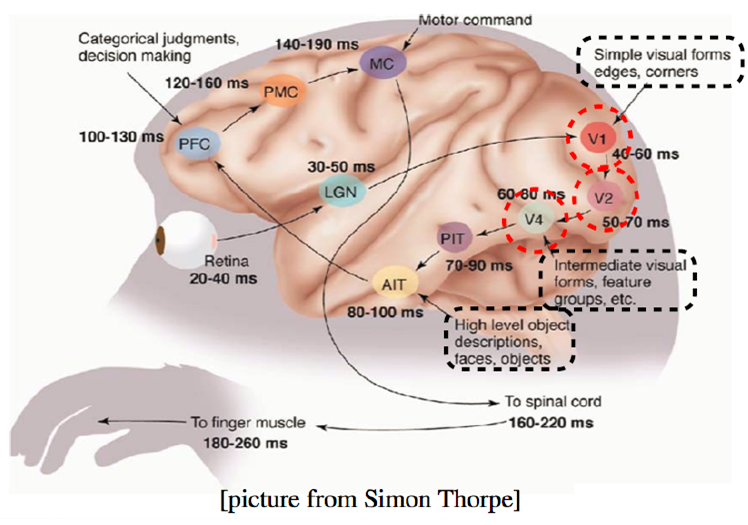
\includegraphics[scale= 0.5]{images/VisualCortex.png}
\end{figure}
\end{overlayarea}

\column{0.5\textwidth}

\begin{overlayarea}{\textwidth}{\textheight}

\onslide<1->{

\begin{figure}
\centering

\includegraphics[scale= 0.3]{images/Layer1Rep.png} 
\end{figure}
}

\onslide<2->{
\begin{figure}
\centering
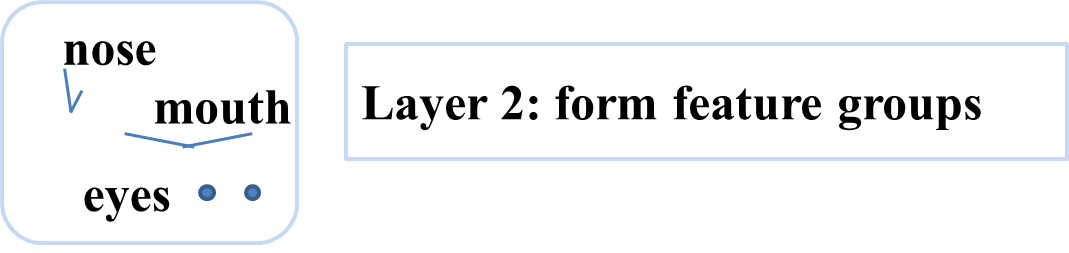
\includegraphics[scale= 0.3]{images/Layer2Rep.png}
\end{figure}
}

\onslide<3->{
\begin{figure}
\centering
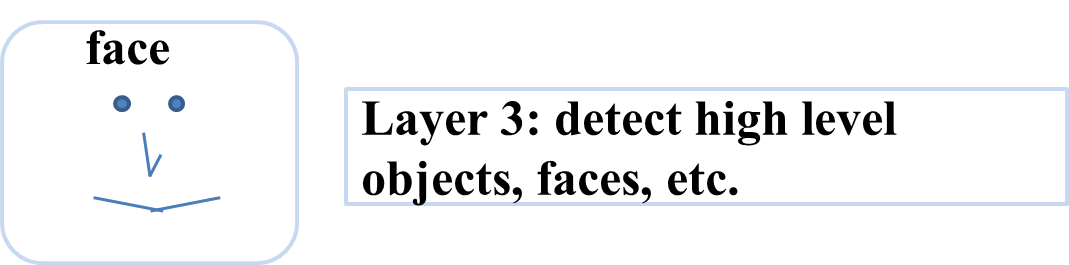
\includegraphics[scale= 0.3]{images/Layer3Rep.png}
\end{figure}
}


\onslide<1->{Sample illustration of hierarchical processing$^*$ \footnotetext{\hspace{-0.3in}$^*$Idea borrowed from Hugo Larochelle's lecture slides}}

\end{overlayarea}
\end{columns}
\end{frame}

\begin{frame}
\begin{block}{Disclaimer}
\begin{itemize}\justifying
\item I understand very little about how the brain works!
\item What you saw so far is an overly simplified explanation of how the brain works!
\item But this explanation suffices for the purpose of this course!
\end{itemize}
\end{block}
\end{frame}

  \begin{frame}
    \myheading{Module 2.2: McCulloch Pitts Neuron}
  \end{frame}


\begin{frame}
\begin{columns}

\column{0.4\textwidth}
\begin{overlayarea}{\textwidth}{\textheight}

\begin{figure}
\begin{tikzpicture}
\node[name=s,shape=circle split,draw=gray!40,line width=0mm,minimum size=2cm] {};

\begin{scope}[on background layer]
\fill[black!50] (s.base) ([xshift=-0mm]s.east) arc (0:180:1cm-0mm)--cycle;
\fill[white!50] (s.base) ([xshift=0mm]s.west) arc (180:360:1cm-0mm)--cycle;  
\end{scope}

\onslide<2->{\node (input0) at (-1.5, -2.0) {$x_1$};}
\onslide<3->{\node (input1) at (-0.75, -2.0) {$x_2$};}
\onslide<4->{\node (input2) at (0, -2.0) {$..$};}
\onslide<4->{\node (input3) at (0.75, -2.0) {$..$};}
\onslide<5->{\node (input4) at (2.25, -2.0) {$x_n \onslide<6->{\in \{0,1\}}$};}

\onslide<9->{\node (output) at (0, 2.0) {$y \in \{0,1\}$};}

\onslide<7->{\node at (0,-0.5) {$g$};}
\onslide<8->{\node at (0,0.5) {$f$};}

\draw [->] (input0) -- (s.240);
\draw [->] (input1) -- (s.255);
\draw [->] (input2) -- (s.270);
\draw [->] (input3) -- (s.285);
\draw [->] (input4) -- (s.300);
\draw [->] (s.90) -- (output);

\end{tikzpicture}
%\caption{A generic computing unit}
\end{figure}

\end{overlayarea}

\column{0.6\textwidth}
\begin{overlayarea}{\textwidth}{\textheight}
\begin{itemize}\justifying
\item McCulloch (neuroscientist) and Pitts (logician) proposed a highly simplified computational model of the neuron (1943)
\item<7-> $g$ aggregates the inputs \onslide<8->{and the function $f$ takes a decision based on this aggregation}
\item<10-> The inputs can be excitatory or inhibitory  
\item<11-> $y = 0$ if any $x_i$ is inhibitory, else

\onslide<12->{
\begin{align*}
\onslide<12->{g(x_1, x_2, ..., x_n) &= g(\mathbf{x}) = \sum_{i=1}^{n} x_i \\}
\onslide<13->{y = f (g(\mathbf{x})) &= 1 \quad if \quad g(\mathbf{x}) \geq \theta \\}
\onslide<14->{&= 0 \quad if \quad g(\mathbf{x}) < \theta}
\end{align*}
}

\vspace{-0.4in}
\item<15-> $\mathbf{\theta}$ is called the thresholding parameter
\item<16-> This is called Thresholding Logic
\end{itemize}
\end{overlayarea}


\end{columns}
\end{frame}


\begin{frame}
Let us implement some boolean functions using this McCulloch Pitts (MP) neuron ...
\end{frame}


\begin{frame}

\begin{columns}

\column{0.33\textwidth}
\begin{overlayarea}{\textwidth}{\textheight}
\begin{center}
\begin{tikzpicture}
\node[name=s,shape=circle split,draw=gray!40,line width=0mm,minimum size=1cm] {};  
\begin{scope}[on background layer]
\fill[black!50] (s.base) ([xshift=-0mm]s.east) arc (0:180:0.5cm-0mm)--cycle;
\fill[white!50] (s.base) ([xshift=0mm]s.west) arc (180:360:0.5cm-0mm)--cycle;  
\end{scope}
\node (input1) at (-0.75, -1.25) {$x_1$};
\node (input2) at (0, -1.25) {$x_2$};
\node (input3) at (0.75, -1.25) {$x_3$};

\node (output) at (0, 1.25) {$y \in \{0,1\}$};

%\node at (0,0.25) {$f$};
\node at (0,-0.25) {$\theta$};

\draw [->] (input1) -- (s.255);
\draw [->] (input2) -- (s.270);
\draw [->] (input3) -- (s.285);
\draw [->] (s.90) -- (output);

\end{tikzpicture}
\captionof{figure}{A McCulloch Pitts unit}

\only<6->{
\begin{tikzpicture}
\node[name=s,shape=circle split,draw=gray!40,line width=0mm,minimum size=1cm] {};  
\begin{scope}[on background layer]
\fill[black!50] (s.base) ([xshift=-0mm]s.east) arc (0:180:0.5cm-0mm)--cycle;
\fill[white!50] (s.base) ([xshift=0mm]s.west) arc (180:360:0.5cm-0mm)--cycle;  
\end{scope}
\node (input1) at (-0.75, -1.25) {$x_1$};
\node (input2) at (0.75, -1.25) {$x_2$};

\node (output) at (0, 1.25) {$y \in \{0,1\}$};

%\node at (0,0.25) {$f$};
\onslide<7->{\node at (0,-0.25) {$1$};}

\draw [->] (input1) -- (s.255);
\draw [o=1pt] (input2) -- (s.285);
\draw [->] (s.90) -- (output);

\end{tikzpicture}
\captionof{figure}{$x_1$ AND $!x_2$$^*$ \footnotetext{$^*$circle at the end indicates inhibitory input: if any inhibitory input is 1 the output will be 0}}
}
\end{center}

\end{overlayarea}

\column{0.33\textwidth}
\begin{overlayarea}{\textwidth}{\textheight}
\begin{center}
\only<2->{
\begin{tikzpicture}
\node[name=s,shape=circle split,draw=gray!40,line width=0mm,minimum size=1cm] {};  
\begin{scope}[on background layer]
\fill[black!50] (s.base) ([xshift=-0mm]s.east) arc (0:180:0.5cm-0mm)--cycle;
\fill[white!50] (s.base) ([xshift=0mm]s.west) arc (180:360:0.5cm-0mm)--cycle;  
\end{scope}
\node (input1) at (-0.75, -1.25) {$x_1$};
\node (input2) at (0, -1.25) {$x_2$};
\node (input3) at (0.75, -1.25) {$x_3$};

\node (output) at (0, 1.25) {$y \in \{0,1\}$};

%\node at (0,0.25) {$f$};
\onslide<3->{\node at (0,-0.25) {3};}

\draw [->] (input1) -- (s.255);
\draw [->] (input2) -- (s.270);
\draw [->] (input3) -- (s.285);
\draw [->] (s.90) -- (output);

\end{tikzpicture}
\captionof{figure}{AND function}
}


\only<8->{
\begin{tikzpicture}
\node[name=s,shape=circle split,draw=gray!40,line width=0mm,minimum size=1cm] {};  
\begin{scope}[on background layer]
\fill[black!50] (s.base) ([xshift=-0mm]s.east) arc (0:180:0.5cm-0mm)--cycle;
\fill[white!50] (s.base) ([xshift=0mm]s.west) arc (180:360:0.5cm-0mm)--cycle;  
\end{scope}
\node (input1) at (-0.75, -1.25) {$x_1$};
\node (input2) at (0.75, -1.25) {$x_2$};

\node (output) at (0, 1.25) {$y \in \{0,1\}$};

%\node at (0,0.25) {$f$};
\onslide<9->{\node at (0,-0.25) {$0$};}

\draw [o=1pt] (input1) -- (s.255);
\draw [o=1pt] (input2) -- (s.285);
\draw [->] (s.90) -- (output);

\end{tikzpicture}
\captionof{figure}{NOR function}
}
\end{center}



\end{overlayarea}

\column{0.33\textwidth}
\begin{overlayarea}{\textwidth}{\textheight}
\begin{center}
\only<4->{
\begin{tikzpicture}
\node[name=s,shape=circle split,draw=gray!40,line width=0mm,minimum size=1cm] {};  
\begin{scope}[on background layer]
\fill[black!50] (s.base) ([xshift=-0mm]s.east) arc (0:180:0.5cm-0mm)--cycle;
\fill[white!50] (s.base) ([xshift=0mm]s.west) arc (180:360:0.5cm-0mm)--cycle;  
\end{scope}
\node (input1) at (-0.75, -1.25) {$x_1$};
\node (input2) at (0, -1.25) {$x_2$};
\node (input3) at (0.75, -1.25) {$x_3$};

\node (output) at (0, 1.25) {$y \in \{0,1\}$};

%\node at (0,0.25) {$f$};
\onslide<5->{\node at (0,-0.25) {$1$};}

\draw [->] (input1) -- (s.255);
\draw [->] (input2) -- (s.270);
\draw [->] (input3) -- (s.285);
\draw [->] (s.90) -- (output);

\end{tikzpicture}
\captionof{figure}{OR function}
}

\only<10->{
\begin{tikzpicture}
\node[name=s,shape=circle split,draw=gray!40,line width=0mm,minimum size=1cm] {};  
\begin{scope}[on background layer]
\fill[black!50] (s.base) ([xshift=-0mm]s.east) arc (0:180:0.5cm-0mm)--cycle;
\fill[white!50] (s.base) ([xshift=0mm]s.west) arc (180:360:0.5cm-0mm)--cycle;  
\end{scope}
\node (input1) at (0.0, -1.25) {$x_1$};
%\node (input2) at (0.75, -1.25) {$x_2$};

\node (output) at (0, 1.25) {$y \in \{0,1\}$};

%\node at (0,0.25) {$f$};
\onslide<11->{\node at (0,-0.25) {$0$};}

\draw [o=1pt] (input1) -- (s.270);
%\draw [o=1pt] (input2) -- (s.285);
\draw [->] (s.90) -- (output);

\end{tikzpicture}
\captionof{figure}{NOT function}
}
\end{center}


\end{overlayarea}

\end{columns}
\end{frame}

\begin{frame}
\begin{itemize}\justifying
\item Can any boolean function be represented using a McCulloch Pitts unit ?
\item<2-> Before answering this question let us first see the geometric interpretation of a MP unit ...
\end{itemize}

\end{frame}


\begin{frame}
\begin{columns}

\column{0.4\textwidth}
\begin{overlayarea}{\textwidth}{\textheight}
\begin{center}
\only<1->{
\begin{tikzpicture}
\node[name=s,shape=circle split,draw=gray!40,line width=0mm,minimum size=1cm] {};  
\begin{scope}[on background layer]
\fill[black!50] (s.base) ([xshift=-0mm]s.east) arc (0:180:0.5cm-0mm)--cycle;
\fill[white!50] (s.base) ([xshift=0mm]s.west) arc (180:360:0.5cm-0mm)--cycle;  
\end{scope}
\node (input1) at (-0.75, -1.25) {$x_1$};
\node (input3) at (0.75, -1.25) {$x_2$};

\node (output) at (0, 1.25) {$y \in \{0,1\}$};

%\node at (0,0.25) {$f$};
\node at (0,-0.25) {1};

\draw [->] (input1) -- (s.255);
\draw [->] (input3) -- (s.285);
\draw [->] (s.90) -- (output);

\end{tikzpicture}
\centering
\captionof{figure}{OR function \\ $x_1 + x_2 = \sum_{i=1}^{2} x_i \geq 1$ }
}

\only<2->{

\begin{tikzpicture}

\draw[thick,->] (0,0) -- (3.5,0);
\draw[thick,->] (0,0) -- (0,3.5);

\onslide<3->{\draw[densely dotted] (-0.3,2.3) -- (2.3,-0.3);}

\node at (3.3, -0.2) {$x_1$};
\node at (-0.2, 3.3) {$x_2$};

\node at (-0.1, -0.3) {$(0,0)$};
\node at (-0.1, 2.3) {$(0,1)$};
\node at (2.0, -0.3) {$(1,0)$};
\node at (2.2, 2.3) {$(1,1)$};
\onslide<3->{\node at (2.7, 1.0) {$x_1 + x_2 = \theta = 1$};}

\filldraw (0,0) circle (2pt);
\filldraw (0,2) circle (2pt);
\filldraw (2,0) circle (2pt);
\filldraw (2,2) circle (2pt);
\end{tikzpicture}
}
\end{center}
\end{overlayarea}

\column{0.6\textwidth}
\begin{overlayarea}{\textwidth}{\textheight}
\begin{itemize}\justifying
\item<4-> A single MP neuron splits the input points (4 points for 2 binary inputs) into two halves
\item<5-> Points lying on or above the line $\sum_{i=1}^{n} x_i - \theta = 0$ and points lying below this line
\item<6-> In other words, all inputs which produce an output 0 will be on one side ($\sum_{i=1}^{n} x_i < \theta$) of the line and all inputs which produce an  output 1 will lie on the other side ($\sum_{i=1}^{n} x_i \geq \theta$) of this line 
\item<7-> Let us convince ourselves about this with a few more examples (if it is not already clear from the math) 
\end{itemize}
\end{overlayarea}
\end{columns}
\end{frame}


\begin{frame}
\begin{columns}

\column{0.4\textwidth}
\begin{overlayarea}{\textwidth}{\textheight}
\begin{center}
\only<1->{
\begin{tikzpicture}
\node[name=s,shape=circle split,draw=gray!40,line width=0mm,minimum size=1cm] {};  
\begin{scope}[on background layer]
\fill[black!50] (s.base) ([xshift=-0mm]s.east) arc (0:180:0.5cm-0mm)--cycle;
\fill[white!50] (s.base) ([xshift=0mm]s.west) arc (180:360:0.5cm-0mm)--cycle;  
\end{scope}
\node (input1) at (-0.75, -1.25) {$x_1$};
\node (input3) at (0.75, -1.25) {$x_2$};

\node (output) at (0, 1.25) {$y \in \{0,1\}$};

%\node at (0,0.25) {$f$};
\node at (0,-0.25) {2};

\draw [->] (input1) -- (s.255);
\draw [->] (input3) -- (s.285);
\draw [->] (s.90) -- (output);

\end{tikzpicture}
\captionof{figure}{AND function \\ $x_1 + x_2 = \sum_{i=1}^{2} x_i \geq 2$ }
}

\only<2->{
\vspace{-0.2in}
\begin{tikzpicture}

\draw[thick,->] (0,0) -- (3.5,0);
\draw[thick,->] (0,0) -- (0,3.5);

\onslide<3->{\draw[densely dotted] (0.0,4.0) -- (4,0);}

\node at (3.3, -0.2) {$x_1$};
\node at (-0.2, 3.3) {$x_2$};

\node at (-0.1, -0.3) {$(0,0)$};
\node at (-0.1, 2.3) {$(0,1)$};
\node at (2.0, -0.3) {$(1,0)$};
\node at (2.2, 2.3) {$(1,1)$};
\onslide<3->{\node at (2.7, 1.0) {$x_1 + x_2 = \theta = 2$};}

\filldraw (0,0) circle (2pt);
\filldraw (0,2) circle (2pt);
\filldraw (2,0) circle (2pt);
\filldraw (2,2) circle (2pt);
\end{tikzpicture}
}
\end{center}
\end{overlayarea}

\column{0.6\textwidth}
\begin{overlayarea}{\textwidth}{\textheight}
\begin{center}
\only<4->{
\begin{tikzpicture}
\node[name=s,shape=circle split,draw=gray!40,line width=0mm,minimum size=1cm] {};  
\begin{scope}[on background layer]
\fill[black!50] (s.base) ([xshift=-0mm]s.east) arc (0:180:0.5cm-0mm)--cycle;
\fill[white!50] (s.base) ([xshift=0mm]s.west) arc (180:360:0.5cm-0mm)--cycle;  
\end{scope}
\node (input1) at (-0.75, -1.25) {$x_1$};
\node (input3) at (0.75, -1.25) {$x_2$};

\node (output) at (0, 1.25) {$y \in \{0,1\}$};

%\node at (0,0.25) {$f$};
\only<5->{\node at (0,-0.25) {0};}

\draw [->] (input1) -- (s.255);
\draw [->] (input3) -- (s.285);
\draw [->] (s.90) -- (output);

\end{tikzpicture}
\captionof{figure}{Tautology (always ON)}
}

\only<6->{

\begin{tikzpicture}

\draw[thick,->] (0,0) -- (3.5,0);
\draw[thick,->] (0,0) -- (0,3.5);

\onslide<7->{\draw[densely dotted] (-2.0,2.0) -- (0.75,-0.75);}

\node at (3.3, -0.2) {$x_1$};
\node at (-0.2, 3.3) {$x_2$};

\node at (-0.1, -0.3) {$(0,0)$};
\node at (-0.1, 2.3) {$(0,1)$};
\node at (2.0, -0.3) {$(1,0)$};
\node at (2.2, 2.3) {$(1,1)$};
\onslide<7->{\node at (-0.1, 1.0) {$x_1 + x_2 = \theta = 0$};}

\filldraw (0,0) circle (2pt);
\filldraw (0,2) circle (2pt);
\filldraw (2,0) circle (2pt);
\filldraw (2,2) circle (2pt);
\end{tikzpicture}
}
\end{center}
\end{overlayarea}
\end{columns}
\end{frame}


\begin{frame}
\begin{columns}

\column{0.5\textwidth}
\begin{overlayarea}{\textwidth}{\textheight}
\begin{center}

\begin{tikzpicture}
\node[name=s,shape=circle split,draw=gray!40,line width=0mm,minimum size=1cm] {};  
\begin{scope}[on background layer]
\fill[black!50] (s.base) ([xshift=-0mm]s.east) arc (0:180:0.5cm-0mm)--cycle;
\fill[white!50] (s.base) ([xshift=0mm]s.west) arc (180:360:0.5cm-0mm)--cycle;  
\end{scope}
\node (input1) at (-0.75, -1.25) {$x_1$};
\node (input2) at (0.0, -1.25) {$x_2$};
\node (input3) at (0.75, -1.25) {$x_3$};

\node (output) at (0, 1.25) {$y \in \{0,1\}$};

%\node at (0,0.25) {$f$};
\node at (1.5,-0.25) {OR};

\node at (0,-0.25) {1};

\draw [->] (input1) -- (s.255);
\draw [->] (input2) -- (s.270);
\draw [->] (input3) -- (s.285);
\draw [->] (s.90) -- (output);


\end{tikzpicture}

\only<2->{
\begin{tikzpicture}

\draw[thick,->] (0,0) -- (3.0,0);
\draw[thick,->] (0,0) -- (0,3.0);
\draw[thick,->] (0,0) -- (-2.0,-2.0);


\node at (2.85, -0.2) {$x_1$};
\node at (-0.2, 2.95) {$x_2$};
\node at (-2.2, -2.0) {$x_3$};

\node at (-0.1, -0.3) {$(0,0,0)$};
\filldraw[fill=red] (0,0) circle (2pt);

\only<5->{\draw[black, fill=gray] (2,0) -- (0,2) -- (-1.2,-1.2) -- (2,0) -- cycle;}

\node at (-0.1, 2.3) {$(0,1,0)$};
\node at (2.0, -0.3) {$(1,0,0)$};
\node at (2.2, 2.3) {$(1,1,0)$};
\node at (-1.2,-1.5) {$(0,0,1)$};
\node at (0.8,-1.5) {$(1,0,1)$};
\node at (-1.0,1.0) {$(0,1,1)$};
\node at (0.8,1.0) {$(1,1,1)$};
\onslide<5->{\node at (3.2, 1.0) {\color{red}{$\mathbf{x_1 + x_2 + x_3 = \mathbf{\theta} = 1}$}};}

\filldraw (0,2) circle (2pt);
\filldraw (2,0) circle (2pt);
\filldraw (2,2) circle (2pt);
\filldraw (-1.2,-1.2) circle (2pt);
\filldraw (-1.2,0.8) circle (2pt);
\filldraw (0.8,-1.2) circle (2pt);


\draw[densely dotted] (0, 2) -- (-1.2,0.8);
\draw[densely dotted] (-1.2,-1.2) -- (-1.2,0.8);
\draw[densely dotted] (0.0,2.0) -- (2,2);
\draw[densely dotted] (2.0,0.0) -- (2,2);
\draw[densely dotted] (0.8,0.8) -- (2,2);
\draw[densely dotted] (0.8,0.8) -- (0.8,-1.2);
\draw[densely dotted] (0.8,-1.2) -- (2,0);
\draw[densely dotted] (-1.2,-1.2) -- (0.8,-1.2);
\draw[densely dotted] (-1.2,0.8) -- (0.8,0.8);


\filldraw (0.8,0.8) circle (2pt);

\end{tikzpicture}
}
\end{center}
\end{overlayarea}

\column{0.5\textwidth}
\begin{overlayarea}{\textwidth}{\textheight}
\begin{itemize}\justifying
\item<1-> What if we have more than 2 inputs?
\item<3-> Well, instead of a line we will have a plane
\item<4-> For the OR function, we want a plane such that the point (0,0,0) lies on one side and the remaining 7 points lie on the other side of the plane

\end{itemize}
\end{overlayarea}
\end{columns}
\end{frame}


\begin{frame}
\begin{block}{The story so far ...}
\onslide<1->{
\begin{itemize}\justifying
\item<1-> A single McCulloch Pitts Neuron can be used to represent boolean functions which are linearly separable
\item<2-> Linear separability (for boolean functions) : There exists a line (plane) such that all inputs which produce a 1 lie on one side of the line (plane) and all inputs which produce a 0 lie on other side of the line (plane)
\end{itemize}
}
\end{block}
\end{frame}

  \begin{frame}
    \myheading{Module 2.3: Perceptron}
  \end{frame}

\begin{frame}
\begin{block}{The story ahead ...}
\onslide<1->{
\begin{itemize}\justifying
\item<1-> What about non-boolean (say, real) inputs ?
\item<2-> Do we always need to hand code the threshold ?
\item<3-> Are all inputs equal ? What if we want to assign more weight (importance) to some inputs ?
\item<4-> What about functions which are not linearly separable ? 
\end{itemize}
}
\end{block}
\end{frame}

\begin{frame}
\begin{columns}

\column{0.4\textwidth}
\begin{overlayarea}{\textwidth}{\textheight}
%\begin{center}
\begin{center}
\onslide<2->{
\tikzstyle{input_neuron}=[circle,draw=red!50,fill=orange!10,thick,minimum size=1mm]
\tikzstyle{hidden_neuron}=[circle,draw=blue!50,fill=blue!10,thick,minimum size=10mm]
\tikzstyle{output_neuron}=[circle,draw=green!50,fill=green!20,thick,minimum size=4mm]

\tikzstyle{input}=[circle,draw=black!50,fill=black!20,thick,minimum size=.2mm]

\begin{tikzpicture}
\node (input0) at (8,-0.1)  {$x_{1}$};
\node (input1) at (9,-0.1)  {$x_{2}$};
\node (input2) at (10,-0.1)  {$..$};
\node (input3) at (11,-0.1)  {$..$};
\node (input4) at (12,-0.1)  {$x_{n}$};

\node [hidden_neuron] (neuron1) at (10,2)  {};


\node (output0)  at (10,3.5) {$y$};

\draw [->] (input0) -- (neuron1);
\draw [->] (input1) -- (neuron1);
\draw [->] (input2) -- (neuron1);
\draw [->] (input3) -- (neuron1);
\draw [->] (input4) -- (neuron1);

\draw [->] (neuron1) -- (output0);

\node (formula)[scale=.8] at (8.1,0.6) {$w_{1}$};
\node (formula)[scale=.8] at (9.1,0.6) {$w_{2}$};
\node (formula)[scale=.8] at (9.8,0.6) {$..$};
\node (formula)[scale=.8] at (10.4,0.6) {$..$};
\node (formula)[scale=.8] at (11.1,0.6) {$w_{n}$};
\end{tikzpicture}
}
%\end{center}

\end{center}
\end{overlayarea}

\column{0.6\textwidth}
\begin{overlayarea}{\textwidth}{\textheight}
\begin{itemize}\justifying
\item<1-> Frank Rosenblatt, an American psychologist, proposed the \textbf{classical perceptron} model (1958)
\item<3-> A more general computational model than McCulloch–Pitts neurons
\item<4-> \textbf{Main differences:} Introduction of numerical weights for inputs and a mechanism for learning these weights 
\item<5-> Inputs are no longer limited to boolean values
\item<6-> Refined and carefully analyzed by Minsky and Papert (1969) - their model is referred to as the \textbf{perceptron} model here
\end{itemize}
\end{overlayarea}
\end{columns}
\end{frame}



\begin{frame}
\begin{columns}

\column{0.4\textwidth}
\begin{overlayarea}{\textwidth}{\textheight}
\begin{center}
\tikzstyle{input_neuron}=[circle,draw=red!50,fill=orange!10,thick,minimum size=1mm]
\tikzstyle{hidden_neuron}=[circle,draw=blue!50,fill=blue!10,thick,minimum size=10mm]
\tikzstyle{output_neuron}=[circle,draw=green!50,fill=green!20,thick,minimum size=4mm]

\tikzstyle{input}=[circle,draw=black!50,fill=black!20,thick,minimum size=.2mm]

\begin{tikzpicture}
\node (input0) at (8,-0.1)  {$x_{1}$};
\node (input1) at (9,-0.1)  {$x_{2}$};
\node (input2) at (10,-0.1)  {$..$};
\node (input3) at (11,-0.1)  {$..$};
\node (input4) at (12,-0.1)  {$x_{n}$};
\onslide<10->{\node (input5) at (7,-0.1)  {$\color{red}{x_{0}=1}$};}

\node [hidden_neuron] (neuron1) at (10,2)  {};


\node (output0)  at (10,3.5) {$y$};

\draw [->] (input0) -- (neuron1);
\draw [->] (input1) -- (neuron1);
\draw [->] (input2) -- (neuron1);
\draw [->] (input3) -- (neuron1);
\draw [->] (input4) -- (neuron1);
\onslide<10->{\draw [->, red] (input5) -- (neuron1);}

\draw [->] (neuron1) -- (output0);

\node (formula)[scale=.8] at (8.4,0.6) {$w_{1}$};
\node (formula)[scale=.8] at (9.1,0.6) {$w_{2}$};
\node (formula)[scale=.8] at (9.8,0.6) {$..$};
\node (formula)[scale=.8] at (10.4,0.6) {$..$};
\node (formula)[scale=.8] at (11.1,0.6) {$w_{n}$};
\onslide<10->{\node (formula)[scale=.8] at (7.2,0.6) {$\color{red}{w_{0} = -\theta}$};}

\end{tikzpicture}

\end{center}

\vspace{-0.2in}
\onslide<7->{A more accepted convention,}
\vspace{-0.1in}
\begin{align*}
\onslide<8->{y &=1 \quad if \sum^{n}_{\color{red}{i=0}} w_i * x_i \geq 0} \\
\onslide<11->{&=0  \quad if \sum^{n}_{\color{red}{i=0}} w_i * x_i < 0} \\
\onslide<9->{where, \quad x_0 &= 1 \quad and \quad w_0 = -\theta}
\end{align*}

\end{overlayarea}

\column{0.6\textwidth}
\begin{overlayarea}{\textwidth}{\textheight}
\begin{align*}
\onslide<2->{y &=1 \quad if \sum^{n}_{\color{red}{i=1}} w_i * x_i \geq \theta} \\
\onslide<3->{&=0  \quad if \sum^{n}_{\color{red}{i=1}} w_i * x_i < \theta}
\onslide<4->{\intertext{Rewriting the above,}}
\onslide<5->{y &=1 \quad if \sum^{n}_{\color{red}{i=1}} w_i * x_i - \theta \geq 0} \\
\onslide<6->{&=0  \quad if \sum^{n}_{\color{red}{i=1}} w_i * x_i -\theta < 0}
\end{align*}
\end{overlayarea}
\end{columns}
\end{frame}

\begin{frame}
We will now try to answer the following questions:
\begin{itemize}\justifying
\item Why are we trying to implement boolean functions?
\item Why do we need weights ?
\item Why is $w_0 = -\theta$ called the bias ?
\end{itemize}
\end{frame}




\begin{frame}
\begin{columns}

\column{0.3\textwidth}
\begin{overlayarea}{\textwidth}{\textheight}
\begin{center}
\tikzstyle{input_neuron}=[circle,draw=red!50,fill=orange!10,thick,minimum size=1mm]
\tikzstyle{hidden_neuron}=[circle,draw=blue!50,fill=blue!10,thick,minimum size=10mm]
\tikzstyle{output_neuron}=[circle,draw=green!50,fill=green!20,thick,minimum size=4mm]

\tikzstyle{input}=[circle,draw=black!50,fill=black!20,thick,minimum size=.2mm]

\begin{tikzpicture}
\node (input5) at (7.5,-0.1)  {$x_{0}=1$};
\node (input0) at (9,-0.1)  {$x_1$};
%\node (input1) at (9,-0.1)  {$x_{2}$};
\node (input2) at (10.5,-0.1)  {$x_2$};
%\node (input3) at (11,-0.1)  {$..$};
\node (input4) at (11.8,-0.1)  {$x_3$};

\node [hidden_neuron] (neuron1) at (10,2)  {};


\node (output0)  at (10,3.5) {$y$};

\draw [->] (input0) -- (neuron1);
%\draw [->] (input1) -- (neuron1);
\draw [->] (input2) -- (neuron1);
%\draw [->] (input3) -- (neuron1);
\draw [->] (input4) -- (neuron1);
\draw [->] (input5) -- (neuron1);

\draw [->] (neuron1) -- (output0);

\node (formula)[scale=.8] at (7.6,0.6) {$w_{0} = -\theta$};
\node (formula)[scale=.8] at (9.0,0.6) {$w_{1}$};
%\node (formula)[scale=.8] at (9.1,0.6) {$w_{2}$};
\node (formula)[scale=.8] at (10.1,0.6) {$w_{2}$};
%\node (formula)[scale=.8] at (10.4,0.6) {$..$};
\node (formula)[scale=.8] at (10.9,0.6) {$w_{3}$};


\end{tikzpicture}

\end{center}

\onslide<3->{
\begin{align*}
x_1 = isActorDamon \\
x_2 = isGenreThriller \\
x_3 = isDirectorNolan \\
\end{align*}
}

\end{overlayarea}

\column{0.7\textwidth}
\begin{overlayarea}{\textwidth}{\textheight}
\only<1-6>{
\begin{itemize}\justifying
\item<1-> Consider the task of predicting whether we would like a movie or not 
\item<2-> Suppose, we base our decision on 3 inputs (binary, for simplicity)  
\item<3-> Based on our past viewing experience (\textbf{data}), we may give a high weight to \textit{isDirectorNolan} as compared to the other inputs
\item<4-> Specifically, even if the actor is not \textit{Matt Damon} and the genre is not \textit{thriller} we would still want to cross the threshold $\theta$ by assigning a high weight to \textit{isDirectorNolan}
%\item<5-> Given the following weight assignments $w_0=-2, w_1=1, w_2=1, w_3=2$, which input configurations will result in an output of 1 (watch movie) ? \onslide<6->{[001, 011, 101, 111, 110]}
\end{itemize}
}

\only<7->{
\begin{itemize}\justifying
\item<7-> $w_0$ is called the bias as it represents the prior (prejudice)
\item<8-> A movie buff may have a very low threshold and may watch any movie irrespective of the genre, actor, director [$\theta = 0$]
\item<9-> On the other hand, a selective viewer may only watch thrillers starring Matt Damon and directed by Nolan [$\theta = 3$]
\item<10-> The weights ($w_1, w_2, ..., w_n$) and the bias ($w_0$) will depend on the data (viewer history in this case)
\end{itemize}
}
\end{overlayarea}
\end{columns}
\end{frame}

\begin{frame}
What kind of functions can be implemented using the perceptron? Any difference from McCulloch Pitts neurons? 
\end{frame}


\begin{frame}
\begin{columns}

\column{0.4\textwidth}
\begin{overlayarea}{\textwidth}{\textheight}

\textbf{McCulloch Pitts Neuron}\\
(assuming no inhibitory inputs)
\begin{align*}
y &=1 \quad if \sum^{n}_{i=0} x_i \geq \theta \\
&=0  \quad if \sum^{n}_{i=0} x_i < \theta \\
\end{align*}

\textbf{Perceptron}
\begin{align*}
y &=1 \quad if \sum^{n}_{i=0} \color{red}{w_i} \color{black}{} * x_i \geq \theta \\
&=0  \quad if \sum^{n}_{i=0} \color{red}{w_i} \color{black}{} * x_i < \theta\\
\end{align*}


\end{overlayarea}

\column{0.6\textwidth}
\begin{overlayarea}{\textwidth}{\textheight}
\begin{itemize}\justifying
\item<2-> From the equations it should be clear that even a perceptron separates the input space into two halves
\item<3-> All inputs which produce a 1 lie on one side and all inputs which produce a 0 lie on the other side
\item<4-> In other words, a single perceptron can only be used to implement linearly separable functions
\item<5-> Then what is the difference? \onslide<6->{The weights (including threshold) can be learned and the inputs can be real valued}
\item<7-> We will first revisit some boolean functions and then see the perceptron learning algorithm (for learning weights) 
\end{itemize}
\end{overlayarea}
\end{columns}
\end{frame}

\begin{frame}
\begin{columns}

\column{0.6\textwidth}
\begin{overlayarea}{\textwidth}{\textheight}

\begin{center}
\begin{table}
\begin{tabular}{cccc}
\hline
$x_1$ & $x_2$ & OR  \\\hline
$0$ & $0$ & \onslide<2->{0} & \onslide<3->{$w_0 + \sum_{i=1}^{2} w_i x_i} \onslide<4->{< 0}$\\
\onslide<5->{$1$} & \onslide<5->{$0$} & \onslide<5->{1} & \onslide<6->{$w_0 + \sum_{i=1}^{2} w_i x_i \geq 0$}\\
\onslide<7->{$0$} & \onslide<7->{$1$} & \onslide<7->{1} & \onslide<8->{$w_0 + \sum_{i=1}^{2} w_i x_i \geq 0$}\\
\onslide<9->{$1$} & \onslide<9->{$1$} & \onslide<9->{1} & \onslide<9->{$w_0 + \sum_{i=1}^{2} w_i x_i \geq 0$}\\
\hline
\end{tabular}
\end{table}


\begin{align*}
\onslide<10->{w_0 + w_1\cdot0 + w_2\cdot0 < 0 &\implies w_0 < 0} \\
\onslide<11->{w_0 + w_1\cdot0 + w_2\cdot1 \geq 0 &\implies w_2 > -w_0} \\
\onslide<12->{w_0 + w_1\cdot1 + w_2\cdot0 \geq 0 &\implies w_1 > -w_0} \\
\onslide<13->{w_0 + w_1\cdot1 + w_2\cdot1 \geq 0 &\implies w_1 + w_2 > -w_0}
\end{align*}

\end{center}

\begin{itemize}\justifying
\item<14-> One possible solution to this set of inequalities is $w_0=-1, w_1=1.1,, w_2=1.1$ (and various other solutions are possible)
%\item Note that we can come up with a similar set of inequalities and found the value of $\theta$ for McCulloch Pitts neuron also
\end{itemize}



\end{overlayarea}

\column{0.4\textwidth}
\begin{overlayarea}{\textwidth}{\textheight}

\onslide<15->{
\begin{tikzpicture}

\draw[thick,->] (0,0) -- (3.5,0);
\draw[thick,->] (0,0) -- (0,3.5);

\onslide<16->{\draw[densely dotted] (-1.2021,3.1111) -- (3.1111,-1.2021);}

\node at (3.3, -0.2) {$x_1$};
\node at (-0.2, 3.3) {$x_2$};

\node at (-0.1, -0.3) {$(0,0)$};
\node at (-0.1, 2.3) {$(0,1)$};
\node at (2.0, -0.3) {$(1,0)$};
\node at (2.2, 2.3) {$(1,1)$};
\onslide<16->{\node at (-0.1, 1.0) {$-1 + 1.1x_1 + 1.1x_2 = 0$};}

\filldraw (0,0) circle (2pt);
\filldraw (0,2) circle (2pt);
\filldraw (2,0) circle (2pt);
\filldraw (2,2) circle (2pt);
\end{tikzpicture}
}

\begin{itemize}\justifying
\item<17-> Note that we can come up with a similar set of inequalities and find the value of $\theta$ for a McCulloch Pitts neuron also \onslide<18->{(Try it!)}
\end{itemize}

\end{overlayarea}



\end{columns}
\end{frame}

  \begin{frame}
    \myheading{Module 2.4: Errors and Error Surfaces}
  \end{frame}


\begin{frame}
\begin{columns}

\column{0.6\textwidth}
\begin{overlayarea}{\textwidth}{\textheight}
\onslide<1->{
\begin{itemize}\justifying
\item<1-> Let us fix the threshold ($-w_0 = 1$) and try different values of $w_1, w_2$
\item<2-> Say, $w_1=-1, w_2=-1$ 
\item<3-> What is wrong with this line? \onslide<4->{We make an error on 1 out of the 4 inputs}
\item<5-> Lets try some more values of $w_1, w_2$ and note how many errors we make

\onslide<6->{
\begin{center}
\begin{table}
\begin{tabular}{ccc}
\hline
$w_1$&$w_2$&errors \\
\hline
\onslide<6->{-1} & \onslide<6->{-1} & \onslide<6->{1}\\
\onslide<7->{1.5} & \onslide<7->{0} & \onslide<7->{1}\\
\onslide<8->{0.45} & \onslide<8->{0.45} & \onslide<8->{3}\\
\hline

\hline
\end{tabular}
\end{table}
\end{center}
}

\item<9-> We are interested in those values of $w_0, w_1, w_2$ which result in 0 error
\item<10-> Let us plot the error surface corresponding to different values of $w_0, w_1, w_2$
\end{itemize}
}
\end{overlayarea}

\column{0.4\textwidth}
\begin{overlayarea}{\textwidth}{\textheight}
\begin{center}
\begin{tikzpicture}

\draw[thick,->] (0,0) -- (3.5,0);
\draw[thick,->] (0,0) -- (0,3.5);

\onslide<1->{\draw[densely dotted] (-1.2021,3.1111) -- (3.1111,-1.2021);}
\onslide<2->{\draw[densely dashed, blue] (-2,1) -- (1,-2);}
\onslide<7->{\draw[densely dashed, blue] (1.33,2.5) -- (1.33,-2.0);}
\onslide<8->{\draw[densely dashed, blue] (4.44,0) -- (0,4.44);}

\node at (3.3, -0.2) {$x_1$};
\node at (-0.2, 3.3) {$x_2$};

\node at (-0.1, -0.3) {$(0,0)$};
\node at (-0.1, 2.3) {$(0,1)$};
\node at (2.0, -0.3) {$(1,0)$};
\node at (2.2, 2.3) {$(1,1)$};
\onslide<1->{\node at (0.1, 2.8) {$-1 + 1.1x_1 + 1.1x_2 = 0$};}
\onslide<2->{\node at (-0.1, -2.0) {$-1 + (-1)x_1 + (-1)x_2 = 0$};}
\onslide<7->{\node at (1, -1.0) {$-1 + (1.5)x_1 + (0)x_2 = 0$};}
\onslide<8->{\node at (1.1, 3.8) {$-1 + (0.45)x_1 + (0.45)x_2 = 0$};}

\filldraw (0,0) circle (2pt);
\filldraw (0,2) circle (2pt);
\filldraw (2,0) circle (2pt);
\filldraw (2,2) circle (2pt);
\end{tikzpicture}
\end{center}

\end{overlayarea}
\end{columns}
\end{frame}

\begin{frame}
\begin{columns}

\column{0.5\textwidth}
\begin{overlayarea}{\textwidth}{\textheight}
\begin{figure}
\includegraphics<4->[scale= 0.5]{images/or_error_surface.png}
\end{figure}

\end{overlayarea}

\column{0.5\textwidth}
\begin{overlayarea}{\textwidth}{\textheight}
\begin{itemize}\justifying
\item<1-> For ease of analysis, we will keep $w_0$ fixed (-1) and plot the error for different values of $w_1, w_2$ 
\item<2-> For a given  $w_0, w_1, w_2$ we will compute $-w_0 + w_1*x_1 + w_2*x_2$ for all combinations of $(x_1, x_2)$ and note down how many errors we make
\item<3-> For the OR function, an error occurs if $(x_1, x_2) = (0,0)$  but $-w_0 + w_1*x_1 + w_2*x_2 \geq 0$ or if $(x_1, x_2) \neq (0,0)$  but $-w_0 + w_1*x_1 + w_2*x_2 < 0$


\item<5-> We are interested in finding an algorithm which finds the values of $w_1, w_2$ which minimize this error
\end{itemize}
\end{overlayarea}
\end{columns}
\end{frame}


  \begin{frame}
    \myheading{Module 2.5: Perceptron Learning Algorithm}
  \end{frame}

\begin{frame}
\begin{itemize}\justifying
\item<1-> We will now see a more principled approach for learning these weights and threshold but before that let us answer this question...
\item<2-> Apart from implementing boolean functions (which does not look very interesting) what can a perceptron be used for ?
\item<3-> Our interest lies in the use of perceptron as a binary classifier. Let us see what this means...
\end{itemize}
\end{frame}

\begin{frame}
\begin{columns}

\column{0.4\textwidth}
\begin{overlayarea}{\textwidth}{\textheight}

\begin{center}

\tikzstyle{input_neuron}=[circle,draw=red!50,fill=orange!10,thick,minimum size=1mm]
\tikzstyle{hidden_neuron}=[circle,draw=blue!50,fill=blue!10,thick,minimum size=10mm]
\tikzstyle{output_neuron}=[circle,draw=green!50,fill=green!20,thick,minimum size=4mm]

\tikzstyle{input}=[circle,draw=black!50,fill=black!20,thick,minimum size=.2mm]
\onslide<5->{
\begin{tikzpicture}
\node (input0) at (7,-0.1)  {$x_{0}=1$};
\node (input1) at (8,-0.1)  {$x_{1}$};
\node (input2) at (9,-0.1)  {$x_{2}$};
\node (input3) at (10,-0.1)  {$..$};
\node (input4) at (11,-0.1)  {$..$};
\node (input5) at (12,-0.1)  {$x_{n}$};

\node [hidden_neuron] (neuron1) at (10,2)  {};


\node (output0)  at (10,3.5) {$y$};

\draw [->] (input0) -- (neuron1);
\draw [->] (input1) -- (neuron1);
\draw [->] (input2) -- (neuron1);
\draw [->] (input3) -- (neuron1);
\draw [->] (input4) -- (neuron1);
\draw [->] (input5) -- (neuron1);

\draw [->] (neuron1) -- (output0);

\onslide<6->{\node (formula)[scale=.8] at (7.2,0.6) {$w_{0} = -\theta$};}
\onslide<6->{\node (formula)[scale=.8] at (8.4,0.6) {$w_{1}$};}
\onslide<6->{\node (formula)[scale=.8] at (9.1,0.6) {$w_{2}$};}
\onslide<6->{\node (formula)[scale=.8] at (9.8,0.6) {$..$};}
\onslide<6->{\node (formula)[scale=.8] at (10.4,0.6) {$..$};}
\onslide<6->{\node (formula)[scale=.8] at (11.1,0.6) {$w_{n}$};}

\end{tikzpicture}
}
\end{center}

\vspace{-0.5in}
\only<4->{
\begin{align*}
x_1 &= isActorDamon \\
x_2 &= isGenreThriller \\
x_3 &= isDirectorNolan \\
x_4 &= imdbRating \textit{(scaled to 0 to 1)}\\
... \quad& \quad...\\
x_n &= criticsRating  \textit{(scaled to 0 to 1)}
\end{align*}
}


\end{overlayarea}

\column{0.6\textwidth}
\begin{overlayarea}{\textwidth}{\textheight}
\begin{itemize}\justifying
\item<1-> Let us reconsider our problem of deciding whether to watch a movie or not
\item<2-> Suppose we are given a list of $m$ movies and a label (class) associated with each movie indicating whether the user liked this movie or not : binary decision
\item<3-> Further, suppose we represent each movie with $n$ features (some boolean, some real valued)
\item<5-> We will assume that the data is linearly separable and we want a perceptron to learn how to make this decision
\item<6-> In other words, we want the perceptron to find the equation of this separating plane (or find the values of $w_0, w_1, w_2, .., w_m$)
\end{itemize}
\end{overlayarea}
\end{columns}
\end{frame}


\begin{frame}
\begin{columns}

\column{0.55\textwidth}
\begin{overlayarea}{\textwidth}{\textheight}

\begin{center}
\begin{algorithm}[H]
\onslide<2->{$P \leftarrow inputs\quad with \quad label \quad 1$\;}
\onslide<3->{$N \leftarrow inputs \quad with \quad label \quad 0$\;}
\onslide<4->{Initialize $\mathbf{w}$ randomly\;}
\onslide<5->{\While{$!convergence$}{
\onslide<7->{Pick random $\mathbf{x} \in P \cup N$ \;}
\onslide<8->{\If{$\mathbf{x} \in P \quad and \quad \sum_{i=0}^{n} w_i * x_i < 0$} {
\onslide<9->{$\mathbf{w} = \mathbf{w} + \mathbf{x}$ \;}
}}
\onslide<10->{\If{$\mathbf{x} \in N \quad and \quad \sum_{i=0}^{n} w_i * x_i \geq 0$} {
\onslide<11->{$\mathbf{w} = \mathbf{w} - \mathbf{x}$ \;}
}}    
}}
\onslide<6->{//the algorithm converges when all the inputs are classified correctly}
\caption{Perceptron Learning Algorithm}
\end{algorithm}
\end{center}

\end{overlayarea}


\column{0.45\textwidth}
\begin{overlayarea}{\textwidth}{\textheight}
\begin{itemize}\justifying
%\item<1-> Let $P$ be the set of all inputs which have a label 1 (watch movie)
%\item<1-> Let $N$ be the set of all inputs which have a label 0 (do not watch movie)
\item<12-> Why would this work ?
\item<13-> To understand why this works we will have to get into a bit of Linear Algebra and a bit of geometry...
\end{itemize}
\end{overlayarea}
\end{columns}
\end{frame}


\begin{frame}
\begin{columns}

\column{0.5\textwidth}
\begin{overlayarea}{\textwidth}{\textheight}
\begin{itemize}\justifying
\item<1-> Consider two vectors $\mathbf{w}$ and $\mathbf{x}$ 
\only<2->{
\begin{align*}
\mathbf{w} &= [w_0, w_1, w_2, ..., w_n] \\
\mathbf{x} &= [1, x_1, x_2, ..., x_n] \\
\onslide<3->{\mathbf{w\cdot x} &= \mathbf{w^Tx} = \sum_{i=0}^{n} w_i*x_i}
\end{align*}
}
\item<4-> We can thus rewrite the perceptron rule as
\only<5->{
\begin{align*}
y &= 1 \quad if \quad \mathbf{w^Tx} \geq 0 \\
&= 0 \quad if \quad \mathbf{w^Tx} < 0 
\end{align*}
}
\end{itemize}

\end{overlayarea}

\column{0.5\textwidth}
\begin{overlayarea}{\textwidth}{\textheight}
\begin{itemize}\justifying
\item<6-> We are interested in finding the line $\mathbf{w^Tx} = 0$ which divides the input space into two halves
\item<7-> Every point ($\mathbf{x}$) on this line satisfies the equation $\mathbf{w^Tx} = 0$
\item<8-> What can you tell about the angle ($\alpha$) between $\mathbf{w}$ and any point ($\mathbf{x}$) which lies on this line ?
\item<9-> The angle is 90$\degree$ ($\because cos \alpha = \frac{w^Tx}{||w||||x||} = 0$)
\item<10-> Since the vector $\mathbf{w}$ is perpendicular to every point on the line it is actually perpendicular to the line itself
\end{itemize}
\end{overlayarea}
\end{columns}
\end{frame}

\begin{frame}
\begin{columns}

\column{0.6\textwidth}
\begin{overlayarea}{\textwidth}{\textheight}
\begin{itemize}\justifying
\item<2-> Consider some points (vectors) which lie in the positive half space of this line (\textit{i.e.}, $\mathbf{w^Tx} \geq 0$)
\item<3-> What will be the angle between any such vector and $\mathbf{w}$ ? \only<4->{Obviously, less than 90$\degree$}
\item<5-> What about points (vectors) which lie in the negative half space of this line (\textit{i.e.}, $\mathbf{w^Tx} < 0$)
\item<6-> What will be the angle between any such vector and $\mathbf{w}$ ? \only<7->{Obviously, greater than 90$\degree$}
\item<8-> Of course, this also follows from the formula ($cos \alpha = \frac{w^Tx}{||w||||x||}$)
\item<9-> Keeping this picture in mind let us revisit the algorithm

\end{itemize}

\end{overlayarea}

\column{0.4\textwidth}
\begin{overlayarea}{\textwidth}{\textheight}
\begin{center}
\begin{tikzpicture}

\draw[thick,->] (0,0) -- (3.5,0);
\draw[thick,->] (0,0) -- (0,3.5);

\onslide<1->{\draw[densely dashed] (-2,2) -- (2,-2);}
\onslide<1->{\draw[-{>[length=3]}] (0,0) -- (2.2, 2.2);}
\onslide<3->{\draw[-{>[length=3]}, blue] (0,0) -- (-0.5, 1.2);}
\onslide<3->{\draw[-{>[length=3]}, blue] (0,0) -- (0.5, 2);}
\onslide<3->{\draw[-{>[length=3]}, blue] (0,0) -- (3, 1);}
\onslide<6->{\draw[-{>[length=3]}, red] (0,0) -- (-1.5, 0.5);}
\onslide<6->{\draw[-{>[length=3]}, red] (0,0) -- (-0.5, -2);}
\onslide<6->{\draw[-{>[length=3]}, red] (0,0) -- (0.5, -2);}


\node at (3.3, -0.2) {$x_1$};
\node at (-0.2, 3.3) {$x_2$};

\onslide<2->{\node at (-0.5, 1.5) {$p_1$};}
\onslide<2->{\node at (0.5, 2.3) {$p_2$};}
\onslide<2->{\node at (3, 1.3) {$p_3$};}
\onslide<5->{\node at (-1.5, 0.2) {$n_1$};}
\onslide<5->{\node at (-0.5, -2.3) {$n_2$};}
\onslide<5->{\node at (0.5, -2.3) {$n_3$};}
%\node at (-0.1, 2.3) {$(0,1)$};
%\node at (2.0, -0.3) {$(1,0)$};
\node at (2.5, 2.5) {$\mathbf{w}$};
\onslide<1->{\node at (-1, 2) {$\mathbf{w^Tx} = 0$};}

\onslide<2->{\filldraw[blue] (-0.5,1.2) circle (2pt);}
\onslide<2->{\filldraw[blue] (0.5,2) circle (2pt);}
\onslide<2->{\filldraw[blue] (3,1) circle (2pt);}
\onslide<5->{\filldraw[red] (-1.5,0.5) circle (2pt);}
\onslide<5->{\filldraw[red] (-0.5,-2) circle (2pt);}
\onslide<5->{\filldraw[red] (0.5,-2) circle (2pt);}
%\filldraw (2,0) circle (2pt);
%\filldraw (2,2) circle (2pt);
\end{tikzpicture}
\end{center}

\end{overlayarea}
\end{columns}
\end{frame}

\begin{frame}
\begin{columns}

\column{0.55\textwidth}
\begin{overlayarea}{\textwidth}{\textheight}
\begin{center}
\begin{algorithm}[H]
$P \leftarrow inputs\quad with \quad label \quad 1$\;
$N \leftarrow inputs \quad with \quad label \quad 0$\;
Initialize $\mathbf{w}$ randomly\;
\While{$!convergence$}{
Pick random $\mathbf{x} \in P \cup N$ \;
\If{$\mathbf{x} \in P \quad and \quad \mathbf{w.x} < 0$} {
$\mathbf{w} = \mathbf{w} + \mathbf{x}$ \;
}
\If{$\mathbf{x} \in N \quad and \quad \mathbf{w.x} \geq 0$} {
$\mathbf{w} = \mathbf{w} - \mathbf{x}$ \;
}    
}
//the algorithm converges when all the inputs are classified correctly
\caption{Perceptron Learning Algorithm}
\end{algorithm}

\vspace{-0.2in}

\scriptsize{
\begin{align*}
cos \alpha = \frac{\mathbf{w}^T\mathbf{x}}{||\mathbf{w}||||\mathbf{x}||} 
\end{align*}
}
\end{center}

\end{overlayarea}

\column{0.45\textwidth}
\begin{overlayarea}{\textwidth}{\textheight}
\begin{itemize}\justifying
\item<2-> For $\mathbf{x} \in P$ if $\mathbf{w.x} < 0$ then it means that the angle ($\alpha$) between this $\mathbf{x}$ and the current $\mathbf{w}$ is greater than 90$\degree$ \onslide<3->{(but we want $\alpha$ to be less than 90$\degree$)}
\item<4-> What happens to the new angle ($\alpha_{new}$) when $\mathbf{w_{new}} = \mathbf{w} + \mathbf{x}$
\onslide<5-> {
\begin{align*}
\onslide<5-> {cos (\alpha_{new}) &\propto \mathbf{w_{new}}^{T}\mathbf{x} \\} 
\onslide<6-> { &\propto (\mathbf{w} + \mathbf{x})^T\mathbf{x} \\}
\onslide<7-> { &\propto \mathbf{w}^T\mathbf{x} + \mathbf{x}^T\mathbf{x} \\}
\onslide<8-> { &\propto cos \alpha + \mathbf{x}^T\mathbf{x} \\}
\onslide<9-> {cos (\alpha_{new}) &> cos \alpha  }
\end{align*}
}
\vspace{-0.35in}
\item<10-> Thus $\alpha_{new}$ will be less than $\alpha$ and this is exactly what we want
\end{itemize}
\end{overlayarea}
\end{columns}
\end{frame}

\begin{frame}
\begin{columns}

\column{0.55\textwidth}
\begin{overlayarea}{\textwidth}{\textheight}
\begin{center}
\begin{algorithm}[H]
$P \leftarrow inputs\quad with \quad label \quad 1$\;
$N \leftarrow inputs \quad with \quad label \quad 0$\;
Initialize $\mathbf{w}$ randomly\;
\While{$!convergence$}{
Pick random $\mathbf{x} \in P \cup N$ \;
\If{$\mathbf{x} \in P \quad and \quad \mathbf{w.x} < 0$} {
$\mathbf{w} = \mathbf{w} + \mathbf{x}$ \;
}
\If{$\mathbf{x} \in N \quad and \quad \mathbf{w.x} \geq 0$} {
$\mathbf{w} = \mathbf{w} - \mathbf{x}$ \;
}    
}
//the algorithm converges when all the inputs are classified correctly
\caption{Perceptron Learning Algorithm}
\end{algorithm}
\vspace{-0.2in}

\scriptsize{
\begin{align*}
cos \alpha = \frac{\mathbf{w}^T\mathbf{x}}{||\mathbf{w}||||\mathbf{x}||} 
\end{align*}
}

\end{center}

\end{overlayarea}

\column{0.45\textwidth}
\begin{overlayarea}{\textwidth}{\textheight}
\begin{itemize}\justifying
\item<2-> For $\mathbf{x} \in N$ if $\mathbf{w.x} \geq 0$ then it means that the angle ($\alpha$) between this $\mathbf{x}$ and the current $\mathbf{w}$ is less than 90$\degree$ \onslide<3->{(but we want $\alpha$ to be greater than 90$\degree$)}
\item<4-> What happens to the new angle ($\alpha_{new}$) when $\mathbf{w_{new}} = \mathbf{w} - \mathbf{x}$
\onslide<5-> {
\begin{align*}
\onslide<5-> {cos (\alpha_{new}) &\propto \mathbf{w_{new}}^{T}\mathbf{x} \\} 
\onslide<6-> { &\propto (\mathbf{w} - \mathbf{x})^T\mathbf{x} \\}
\onslide<7-> { &\propto \mathbf{w}^T\mathbf{x} - \mathbf{x}^T\mathbf{x} \\}
\onslide<8-> { &\propto cos \alpha - \mathbf{x}^T\mathbf{x} \\}
\onslide<9-> {cos (\alpha_{new}) &< cos \alpha  }
\end{align*}
}
\vspace{-0.35in}
\item<10-> Thus $\alpha_{new}$ will be greater than $\alpha$ and this is exactly what we want
\end{itemize}
\end{overlayarea}
\end{columns}
\end{frame}

\begin{frame}
\begin{itemize}\justifying
\item<1-> We will now see this algorithm in action for a toy dataset
\end{itemize}
\end{frame}

\begin{frame}
\begin{columns}

\column{0.4\textwidth}
\begin{overlayarea}{\textwidth}{\textheight}
\begin{center}
\begin{tikzpicture}

\draw[thick,->] (0,0) -- (3.5,0);
\draw[thick,->] (0,0) -- (0,3.5);

%\draw[densely dashed] (-2,2) -- (2,-2);
%\draw[-{>[length=3]}] (0,0) -- (2.2, 2.2);
\draw[-{>[length=3]}, blue] (0,0) -- (-0.5, 1.2);
\draw[-{>[length=3]}, blue] (0,0) -- (0.5, 2);
\draw[-{>[length=3]}, blue] (0,0) -- (3, 1);
\draw[-{>[length=3]}, red] (0,0) -- (-1.5, 0.5);
\draw[-{>[length=3]}, red] (0,0) -- (-0.5, -2);
\draw[-{>[length=3]}, red] (0,0) -- (0.5, -2);


\node at (3.3, -0.2) {$x_1$};
\node at (-0.2, 3.3) {$x_2$};

\node at (-0.5, 1.5) {$p_1$};
\node at (0.5, 2.3) {$p_2$};
\node at (3, 1.3) {$p_3$};
\node at (-1.5, 0.2) {$n_1$};
\node at (-0.5, -2.3) {$n_2$};
\node at (0.5, -2.3) {$n_3$};
%\node at (-0.1, 2.3) {$(0,1)$};
%\node at (2.0, -0.3) {$(1,0)$};
%\node at (2.5, 2.5) {$\mathbf{w}$};
%\node at (-1, 2) {$\mathbf{w^Tx} = 0$};

\filldraw[blue] (-0.5,1.2) circle (2pt);
\filldraw[blue] (0.5,2) circle (2pt);
\filldraw[blue] (3,1) circle (2pt);
\filldraw[red] (-1.5,0.5) circle (2pt);
\filldraw[red] (-0.5,-2) circle (2pt);
\filldraw[red] (0.5,-2) circle (2pt);

\onslide<1->{\draw[-{>[length=3]}] (0,0) -- (-2.000000, -2.000000);}
\onslide<5->{\draw[-{>[length=3]}] (0,0) -- (-2.500000, -0.800000);}
\onslide<7->{\draw[-{>[length=3]}] (0,0) -- (-2.000000, 1.200000);}
\onslide<9->{\draw[-{>[length=3]}] (0,0) -- (-0.500000, 0.700000);}
\onslide<11->{\draw[-{>[length=3]}] (0,0) -- (-0.500000, 0.700000);}
\onslide<13->{\draw[-{>[length=3]}] (0,0) -- (-0.500000, 0.700000);}
\onslide<15->{\draw[-{>[length=3]}] (0,0) -- (2.500000, 1.700000);}
\onslide<17->{\draw[-{>[length=3]}] (0,0) -- (2.500000, 1.700000);}
\onslide<19->{\draw[-{>[length=3]}] (0,0) -- (2.500000, 1.700000);}
\onslide<21->{\draw[-{>[length=3]}] (0,0) -- (2.500000, 1.700000);}
\onslide<23->{\draw[-{>[length=3]}] (0,0) -- (2.500000, 1.700000);}
\onslide<25->{\draw[-{>[length=3]}] (0,0) -- (2.500000, 1.700000);}

%\filldraw (2,0) circle (2pt);
%\filldraw (2,2) circle (2pt);
\end{tikzpicture}
\end{center}



\end{overlayarea}

\column{0.6\textwidth}
\begin{overlayarea}{\textwidth}{\textheight}
\begin{itemize}\justifying
\item<1-> We initialized $\mathbf{w}$ to a random value
\item<2-> We observe that currently, $\mathbf{w}\cdot \mathbf{x} < 0$ ($\because$ angle $>$ 90$\degree$) for all the positive points and  $ \mathbf{w} \cdot \mathbf{x} \geq 0$ ($\because$ angle $<$ 90$\degree$) for all the negative points (the situation is exactly oppsite of what we actually want it to be)
\item<3-> We now run the algorithm by randomly going over the points
\only<4-5>{\item Randomly pick a point (say, $p_1$), apply correction $\mathbf{w} = \mathbf{w} + \mathbf{x}$ $\because \mathbf{w\cdot x < 0}$ (you can check the angle visually) }
\only<6-7>{\item Randomly pick a point (say, $p_2$), apply correction $\mathbf{w} = \mathbf{w} + \mathbf{x}$ $\because \mathbf{w\cdot x < 0}$ (you can check the angle visually) }
\only<8-9>{\item Randomly pick a point (say, $n_1$), apply correction $\mathbf{w} = \mathbf{w} - \mathbf{x}$ $\because \mathbf{w\cdot x \geq 0}$ (you can check the angle visually) }
\only<10-11>{\item Randomly pick a point (say, $n_3$), no correction needed $\because \mathbf{w\cdot x < 0}$ (you can check the angle visually) }
\only<12-13>{\item Randomly pick a point (say, $n_2$), no correction needed $\because \mathbf{w\cdot x < 0}$ (you can check the angle visually)}
\only<14-15>{\item Randomly pick a point (say, $p_3$), apply correction $\mathbf{w} = \mathbf{w} + \mathbf{x}$ $\because \mathbf{w\cdot x < 0}$ (you can check the angle visually) }
\only<16-17>{\item Randomly pick a point (say, $p_1$), no correction needed $\because \mathbf{w\cdot x \geq 0}$ (you can check the angle visually)} 
\only<18-19>{\item Randomly pick a point (say, $p_2$), no correction needed $\because \mathbf{w\cdot x \geq 0}$ (you can check the angle visually)}
\only<20-21>{\item Randomly pick a point (say, $n_1$), no correction needed $\because \mathbf{w\cdot x < 0}$ (you can check the angle visually)}
\only<22-23>{\item Randomly pick a point (say, $n_3$), no correction needed $\because \mathbf{w\cdot x < 0}$ (you can check the angle visually)}
\only<24-25>{\item Randomly pick a point (say, $n_2$), no correction needed $\because \mathbf{w\cdot x < 0}$ (you can check the angle visually)}
\only<26>{\item Randomly pick a point (say, $p_3$), no correction needed $\because \mathbf{w\cdot x \geq 0}$ (you can check the angle visually)} 
\item<27> The algorithm has converged
\end{itemize}
\end{overlayarea}
\end{columns}
\end{frame}

  \begin{frame}
    \myheading{Module 2.6: Proof of Convergence}
  \end{frame}

\begin{frame}
\begin{itemize}\justifying
\item<1-> Now that we have some faith and intuition about why the algorithm works, we will see a more formal proof of convergence ...
\end{itemize}
\end{frame}

\begin{frame}
\begin{block}{Theorem}
\textbf{Definition:} Two sets $P$ and $N$ of points in an $n$-dimensional space are called absolutely linearly separable if \onslide<2->{$n$ + 1 real numbers $w_0, w_1, . . . , w_n$ exist} \onslide<3->{such that every point $(x_1, x_2, . . . , x_n) \in  P$ satisfies $\sum_{i=1}^{n} w_i * x_i > w_0$} \onslide<4->{and every point $(x_1, x_2, . . . , x_n) \in  N$ satisfies $\sum_{i=1}^{n} w_i * x_i < w_0$.} \\
\vspace{0.2in}
\onslide<5->{\textbf{Proposition:}} \onslide<6->{If the sets $P$ and $N$ are finite and linearly separable,} \onslide<7->{the perceptron learning algorithm updates the weight vector $\mathbf{w}_t$ a finite number of times.} \onslide<8->{In other words: if the vectors in $P$ and $N$ are tested cyclically one after the other,} \onslide<9->{a weight vector $\mathbf{w}_t$ is found after a finite number of steps $t$ which can separate the two sets.} \\
\vspace{0.2in}
\onslide<10->{\textbf{Proof:} On the next slide}
\end{block}
\end{frame}


\begin{frame}
\begin{columns}

\column{0.4\textwidth}
\begin{overlayarea}{\textwidth}{\textheight}
\textbf{Setup:}
\begin{itemize}\justifying
\item<1-> If $x \in N$ then -$x \in P$ ($\because w^Tx < 0 \implies w^T(-x) \geq 0 $) 
\item<2-> We can thus consider a single set $P' = P \cup N^-$ and for every element $p \in P'$ ensure that $w^Tp \geq 0$
\item<12-> Further we will normalize all the $p$'s so that $||p|| = 1$ (notice that this does not affect the solution $\because if \quad w^T \frac{p}{||p||} \geq 0$ then $w^Tp \geq 0$)  
\item<14-> Let $w^*$ be the normalized solution vector (we know one exists as the data is linearly separable)
\end{itemize}

\end{overlayarea}

\column{0.6\textwidth}
\begin{overlayarea}{\textwidth}{\textheight}

\begin{center}
\small{
\onslide<3->{
\begin{algorithm}[H]
\onslide<3->{$P \leftarrow inputs\quad with \quad label \quad 1$\;}
\onslide<4->{$N \leftarrow inputs \quad with \quad label \quad 0$\;}
\onslide<5->{$N^- \textit{contains negations of all points in N}$\;}
\onslide<6->{$P' \leftarrow P \cup N^-$\;}
\onslide<7->{Initialize $\mathbf{w}$ randomly\;}
\onslide<8->{\While{$!convergence$}{
\onslide<9->{Pick random $\mathbf{p} \in P'$ \;}
\onslide<13->{$\mathbf{p} \leftarrow \frac{p}{||p||} \quad (\textit{so now,} ||p||=1)$ \;}
\onslide<10->{\If{$\mathbf{w.p} < 0$} {
\onslide<11->{$\mathbf{w} = \mathbf{w} + \mathbf{p}$ \;}
}}
}}
\onslide<8->{//the algorithm converges when all the inputs are classified correctly\\}
\onslide<11->{//notice that we do not need the other \textbf{if} condition because by construction we want all points in $P'$ to lie in the positive half space $\mathbf{w.p} \geq 0$}
\caption{Perceptron Learning Algorithm}
\end{algorithm}
}}
\end{center}


\end{overlayarea}
\end{columns}
\end{frame}


\begin{frame}
\begin{columns}

\column{0.42\textwidth}
\begin{overlayarea}{\textwidth}{\textheight}
\textbf{Observations:}
\begin{itemize}\justifying
\item $w^*$ is some optimal solution which exists but we don't know what it is
\item<13-> We do not make a correction at every time-step 
\item<14-> We make a correction only if $w^T\cdot p_i \leq 0$ at that time step
\item<15-> So at time-step $t$ we would have made only $k$ ($\leq t$) corrections  
\item<16-> Every time we make a correction a quantity  $\delta$ gets added to the numerator
\item<17-> So by time-step $t$, a quantity $k\delta$ gets added to the numerator
\end{itemize}

\end{overlayarea}

\column{0.58\textwidth}
\begin{overlayarea}{\textwidth}{\textheight}
\textbf{Proof:}
\begin{itemize}\justifying
\item<2-> Now suppose at time step $t$ we inspected the point $p_i$ and found that $w^T\cdot p_i \leq 0$
\item<3-> We make a correction $w_{t+1} = w_t + p_i$
\item<4-> Let $\beta$ be the angle between $w^*$ and $w_{t+1}$
\vspace{-0.1in}
\begin{align*}
\onslide<5->{cos \beta &= \frac{w^*\cdot w_{t+1}}{||w_{t+1}||} \\}
\onslide<6->{Numerator &= w^*\cdot w_{t+1} \onslide<7->{= w^*\cdot (w_{t} + p_i) \\}}
\onslide<8->{&= w^*\cdot w_{t} + w^*\cdot p_i \\}
\onslide<9->{&\geq w^*\cdot w_{t} + \delta \quad (\delta = min\{w^*\cdot p_i | \forall i \}) \\}
\onslide<10->{&\geq w^*\cdot (w_{t-1} + p_j) + \delta \\}
\onslide<11->{&\geq w^*\cdot w_{t-1} + w^*\cdot p_j + \delta \\}
\onslide<12->{&\geq w^*\cdot w_{t-1} + 2\delta \\}
\onslide<18->{&\geq w^*\cdot w_{0} + (k)\delta \quad (\textit {By induction})}
\end{align*}

\end{itemize}
\end{overlayarea}
\end{columns}
\end{frame}


\begin{frame}
\begin{columns}

\column{1.0\textwidth}
\begin{overlayarea}{\textwidth}{\textheight}
\textbf{Proof (continued:)}
\begin{align*}
\onslide<1->{\textit{So far we have,}\quad w^T\cdot p_i &\leq 0 \quad \textit{(and hence we made the correction)} \\}
\onslide<2->{cos \beta &= \frac{w^*\cdot w_{t+1}}{||w_{t+1}||} \quad (\textit{by definition}) \\}
\onslide<3->{Numerator &\geq w^*\cdot w_{0} + k\delta \quad (\textit {proved by induction}) \\}
\onslide<4->{Denominator^2 &= ||w_{t+1}||^2 \\}
\onslide<5->{&= (w_t + p_i)\cdot(w_t + p_i) \\}
\onslide<6->{&= ||w_t||^2 + 2 w_t \cdot p_i + ||p_i||^2) \\}
\onslide<7->{&\leq ||w_t||^2 + ||p_i||^2 \quad (\because w_t \cdot p_i \leq 0) \\}
\onslide<8->{&\leq ||w_t||^2 + 1 \quad (\because ||p_i||^2 = 1) \\}
\onslide<9->{&\leq (||w_{t-1}||^2 + 1) + 1 \\}
\onslide<10->{&\leq ||w_{t-1}||^2 + 2 \\}
\onslide<11->{&\leq ||w_{0}||^2 + (k) \quad (\textit {By same observation that we made about $\delta$})}
\end{align*}
\end{overlayarea}

\end{columns}
\end{frame}


\begin{frame}
\begin{columns}

\column{1.0\textwidth}
\begin{overlayarea}{\textwidth}{\textheight}
\textbf{Proof (continued:)}
\begin{align*}
\onslide<1->{\textit{So far we have,}\quad w^T\cdot p_i &\leq 0 \quad \textit{(and hence we made the correction)} \\}
\onslide<1->{cos \beta &= \frac{w^*\cdot w_{t+1}}{||w_{t+1}||} \quad (\textit{by definition}) \\}
\onslide<1->{Numerator &\geq w^*\cdot w_{0} + k\delta \quad (\textit {proved by induction}) \\}
\onslide<1->{Denominator^2 &\leq ||w_{0}||^2 + k \quad (\textit {By same observation that we made about $\delta$}) \\}
\onslide<2->{cos \beta &\geq \frac{w^*\cdot w_{0} + k\delta}{\sqrt{||w_{0}||^2 + k}} \\}
\end{align*}
\vspace{-0.5in}
\begin{itemize}\justifying
\item<3-> $cos \beta$ thus grows proportional to $\sqrt{k}$
\item<4-> As $k$ (number of corrections) increases $cos \beta$ can become arbitrarily large
\item<5-> But since $cos \beta \leq 1$, $k$ must be bounded by a maximum number
\item<6-> Thus, there can only be a finite number of corrections ($k$) to $w$ and the algorithm will converge!
\end{itemize}

\end{overlayarea}

\end{columns}
\end{frame}


\begin{frame}
\begin{block}{Coming back to our questions ...}
\onslide<1->{
\begin{itemize}\justifying
\item What about non-boolean (say, real) inputs ? \onslide<2->{\color{red}{Real valued inputs are allowed in perceptron}} \color{black}
\item Do we always need to hand code the threshold ? \onslide<3->{\color{red}{No, we can learn the threshold}} \color{black}
\item Are all inputs equal ? What if we want to assign more weight (importance) to some inputs ? \onslide<4->{\color{red}{A perceptron allows weights to be assigned to inputs}} \color{black}
\item What about functions which are not linearly separable ? \onslide<5->{\color{red}{Not possible with a single perceptron but we will see how to handle this ..}} \color{black}
\end{itemize}
}
\end{block}
\end{frame}

  \begin{frame}
    \myheading{Module 2.7: Linearly Separable Boolean Functions}
  \end{frame}


\begin{frame}
\begin{itemize}\justifying
\item<1-> So what do we do about functions which are not linearly separable ?
\item<2-> Let us see one such simple boolean function first ?
\end{itemize}
\end{frame}


\begin{frame}
\begin{columns}

\column{0.6\textwidth}
\begin{overlayarea}{\textwidth}{\textheight}

\begin{center}
\begin{table}
\begin{tabular}{cccc}
\hline
$x_1$ & $x_2$ & XOR  \\\hline
$0$ & $0$ & 0 & $w_0 + \sum_{i=1}^{2} w_i x_i < 0$\\
$1$ & $0$ & 1 & $w_0 + \sum_{i=1}^{2} w_i x_i \geq 0$\\
$0$ & $1$ & 1 & $w_0 + \sum_{i=1}^{2} w_i x_i \geq 0$\\
$1$ & $1$ & 0 & $w_0 + \sum_{i=1}^{2} w_i x_i < 0$\\
\hline

\end{tabular}
\end{table}


\begin{align*}
\onslide<2->{w_0 + w_1\cdot0 + w_2\cdot0 < 0 &\implies w_0 < 0} \\
\onslide<3->{w_0 + w_1\cdot0 + w_2\cdot1 \geq 0 &\implies w_2 > -w_0} \\
\onslide<4->{w_0 + w_1\cdot1 + w_2\cdot0 \geq 0 &\implies w_1 > -w_0} \\
\onslide<5->{w_0 + w_1\cdot1 + w_2\cdot1 \geq 0 &\implies w_1 + w_2 < -w_0}
\end{align*}

\end{center}

\begin{itemize}\justifying
\item<6-> The fourth condition contradicts conditions 2 and 3
\item<7-> Hence we cannot have a solution to this set of inequalities

%\item Note that we can come up with a similar set of inequalities and found the value of $\theta$ for McCulloch Pitts neuron also
\end{itemize}



\end{overlayarea}

\column{0.4\textwidth}
\begin{overlayarea}{\textwidth}{\textheight}

\onslide<7->{
\begin{tikzpicture}

\draw[thick,->] (0,0) -- (3.5,0);
\draw[thick,->] (0,0) -- (0,3.5);

%\onslide<8->{\draw[densely dotted] (-1.2021,3.1111) -- (3.1111,-1.2021);}

\node at (3.3, -0.2) {$x_1$};
\node at (-0.2, 3.3) {$x_2$};

\node at (-0.1, -0.3) {$(0,0)$};
\node at (-0.1, 2.3) {$(0,1)$};
\node at (2.0, -0.3) {$(1,0)$};
\node at (2.2, 2.3) {$(1,1)$};
%\onslide<8->{\node at (-0.1, 1.0) {$-1 + 1.1x_1 + 1.1x_2 = 0$};}

\filldraw[blue] (0,0) circle (2pt);
\filldraw[red] (0,2) circle (2pt);
\filldraw[red] (2,0) circle (2pt);
\filldraw[blue] (2,2) circle (2pt);
\end{tikzpicture}
}

\begin{itemize}\justifying
\item<8-> And indeed you can see that it is impossible to draw a line which separates the red points from the blue points
\end{itemize}

\end{overlayarea}

\end{columns}
\end{frame}

\begin{frame}
\begin{columns}

\column{0.4\textwidth}
\begin{overlayarea}{\textwidth}{\textheight}
\begin{tikzpicture}
\filldraw[red] (1.717248,1.148263) circle (2pt);
\filldraw[blue] (1.022337,1.844630) circle (2pt);
\filldraw[blue] (0.929218,1.449012) circle (2pt);
\filldraw[red] (1.256599,1.328157) circle (2pt);
\filldraw[blue] (1.917421,1.041134) circle (2pt);
\filldraw[blue] (1.552910,0.757361) circle (2pt);
\filldraw[red] (0.476688,0.993158) circle (2pt);
\filldraw[blue] (1.139669,1.889055) circle (2pt);
\filldraw[red] (1.994183,1.472244) circle (2pt);
\filldraw[red] (0.611827,0.938297) circle (2pt);
\filldraw[blue] (1.954791,0.598560) circle (2pt);
\filldraw[red] (0.113127,1.025315) circle (2pt);
\filldraw[blue] (1.547272,1.235639) circle (2pt);
\filldraw[blue] (1.667688,0.664851) circle (2pt);
\filldraw[blue] (0.108270,0.066074) circle (2pt);
\filldraw[red] (1.551238,0.091185) circle (2pt);
\filldraw[red] (0.550644,0.461861) circle (2pt);
\filldraw[blue] (1.326191,1.171462) circle (2pt);
\filldraw[red] (0.285269,0.166320) circle (2pt);
\filldraw[blue] (0.645487,1.900755) circle (2pt);
\filldraw[red] (0.715271,0.514446) circle (2pt);
\filldraw[blue] (0.239037,0.110620) circle (2pt);
\filldraw[blue] (1.707163,1.213513) circle (2pt);
\filldraw[blue] (0.663682,1.796715) circle (2pt);
\filldraw[red] (0.512817,0.075660) circle (2pt);
\filldraw[blue] (1.542905,0.897760) circle (2pt);
\filldraw[blue] (1.928409,0.514645) circle (2pt);
\filldraw[blue] (0.430763,1.999726) circle (2pt);
\filldraw[red] (0.411993,0.218422) circle (2pt);
\filldraw[red] (0.951387,0.725352) circle (2pt);
\filldraw[red] (0.001601,1.490619) circle (2pt);
\filldraw[red] (0.983530,0.364934) circle (2pt);
\filldraw[red] (0.612532,0.194346) circle (2pt);
\filldraw[blue] (1.217355,1.773029) circle (2pt);
\filldraw[red] (0.398657,0.261244) circle (2pt);
\filldraw[blue] (0.452156,1.890002) circle (2pt);
\filldraw[red] (0.458527,0.384611) circle (2pt);
\filldraw[blue] (1.977895,1.687690) circle (2pt);
\filldraw[blue] (0.217980,0.748811) circle (2pt);
\filldraw[red] (0.075486,1.486788) circle (2pt);
\filldraw[blue] (1.872187,1.761516) circle (2pt);
\filldraw[blue] (1.142016,1.716686) circle (2pt);
\filldraw[blue] (1.411278,1.734101) circle (2pt);
\filldraw[blue] (1.951329,1.101424) circle (2pt);
\filldraw[red] (0.543241,0.052208) circle (2pt);

\draw[thick,->] (-0.5,-0.5) -- (3.5,-0.5);
\draw[thick,->] (-0.5,-0.5) -- (-0.5,3.5);

\if 0
\onslide<1->{\draw[-{>[length=3]}] (0,0) -- (-1.890340, 3.855113);}
\onslide<1->{\draw[-{>[length=3]}] (0,0) -- (-3.146939, 2.526956);}
\onslide<1->{\draw[-{>[length=3]}] (0,0) -- (-1.594029, 3.284317);}
\onslide<1->{\draw[-{>[length=3]}] (0,0) -- (-3.311277, 2.136054);}
\onslide<1->{\draw[-{>[length=3]}] (0,0) -- (-2.288940, 3.980684);}
\onslide<1->{\draw[-{>[length=3]}] (0,0) -- (-0.371519, 5.021818);}
\onslide<1->{\draw[-{>[length=3]}] (0,0) -- (-0.371519, 5.021818);}
\onslide<1->{\draw[-{>[length=3]}] (0,0) -- (-1.628118, 3.693661);}
\onslide<1->{\draw[-{>[length=3]}] (0,0) -- (-1.628118, 3.693661);}
\onslide<1->{\draw[-{>[length=3]}] (0,0) -- (-3.345366, 2.545398);}
\onslide<1->{\draw[-{>[length=3]}] (0,0) -- (-3.345366, 2.545398);}
\onslide<1->{\draw[-{>[length=3]}] (0,0) -- (-1.427945, 3.586532);}
\onslide<1->{\draw[-{>[length=3]}] (0,0) -- (-1.427945, 3.586532);}
\onslide<1->{\draw[-{>[length=3]}] (0,0) -- (-2.684544, 2.258375);}
\onslide<1->{\draw[-{>[length=3]}] (0,0) -- (-1.131634, 3.015736);}
\onslide<1->{\draw[-{>[length=3]}] (0,0) -- (-2.848882, 1.867473);}
\fi 

\end{tikzpicture}

\only<3->{
\begin{tikzpicture}
\foreach \a in {1,2,...,18}{
\draw (\a*360/18: 1cm) node{\color{blue}{$+$}};
}
\foreach \a in {1,2,...,36}{
\draw (\a*360/36: 1.5cm) node{\color{red}{$o$}};
}

\draw[thick,->] (-1.6,-1.6) -- (2.5,-1.6);
\draw[thick,->] (-1.6,-1.6) -- (-1.6,2.5);

\end{tikzpicture}
}

\end{overlayarea}

\column{0.6\textwidth}
\begin{overlayarea}{\textwidth}{\textheight}
\begin{itemize}\justifying
\item<1-> Most real world data is not linearly separable and will always contain some outliers
\item<2-> In fact, sometimes there may not be any outliers but still the data may not be linearly separable 
\item<3-> We need computational units (models) which can deal with such data
\item<4-> While a single perceptron cannot deal with such data, we will show that a network of perceptrons can indeed deal with such data
\end{itemize}
\end{overlayarea}
\end{columns}
\end{frame}


\begin{frame}
\begin{itemize}\justifying
\item<1-> Before seeing how a network of perceptrons can deal with linearly inseparable data, we will discuss boolean functions in some more detail ...
\end{itemize}
\end{frame}


\begin{frame}
\begin{itemize}\justifying
\item How many boolean functions can you design from 2 inputs ?
\item<2-> Let us begin with some easy ones which you already know ..
\onslide<3->{
\footnotesize{
\begin{table}
\begin{tabular}{cccccccccccccccccc}
\hline

\onslide<3->{$x_1$}&\onslide<3->{$x_2$}&\onslide<4->{$f_1$}&\onslide<6->{$f_2$}&\onslide<8->{$f_3$}&\onslide<9->{$f_4$}&\onslide<10->{$f_5$}&\onslide<11->{$f_6$}&\onslide<12->{$f_7$}&\onslide<7->{$f_8$}&\onslide<13->{$f_9$}&\onslide<14->{$f_{10}$}&\onslide<15->{$f_{11}$}&\onslide<16->{$f_{12}$}&\onslide<17->{$f_{13}$}&\onslide<18->{$f_{14}$}&\onslide<19->{$f_{15}$}&\onslide<5->{$f_{16}$}\\
\hline
\onslide<3->{0}&\onslide<3->{0}&\onslide<4->{0}&\onslide<6->{0}&\onslide<8->{0}&\onslide<9->{0}&\onslide<10->{0}&\onslide<11->{0}&\onslide<12->{0}&\onslide<7->{0}&\onslide<13->{1}&\onslide<14->{1}&\onslide<15->{1}&\onslide<16->{1}&\onslide<17->{1}&\onslide<18->{1}&\onslide<19->{1}&\onslide<5->{1}\\
\onslide<3->{0}&\onslide<3->{1}&\onslide<4->{0}&\onslide<6->{0}&\onslide<8->{0}&\onslide<9->{0}&\onslide<10->{1}&\onslide<11->{1}&\onslide<12->{1}&\onslide<7->{1}&\onslide<13->{0}&\onslide<14->{0}&\onslide<15->{0}&\onslide<16->{0}&\onslide<17->{1}&\onslide<18->{1}&\onslide<19->{1}&\onslide<5->{1}\\
\onslide<3->{1}&\onslide<3->{0}&\onslide<4->{0}&\onslide<6->{0}&\onslide<8->{1}&\onslide<9->{1}&\onslide<10->{0}&\onslide<11->{0}&\onslide<12->{1}&\onslide<7->{1}&\onslide<13->{0}&\onslide<14->{0}&\onslide<15->{1}&\onslide<16->{1}&\onslide<17->{0}&\onslide<18->{0}&\onslide<19->{1}&\onslide<5->{1}\\
\onslide<3->{1}&\onslide<3->{1}&\onslide<4->{0}&\onslide<6->{1}&\onslide<8->{0}&\onslide<9->{1}&\onslide<10->{0}&\onslide<11->{1}&\onslide<12->{0}&\onslide<7->{1}&\onslide<13->{0}&\onslide<14->{1}&\onslide<15->{0}&\onslide<16->{1}&\onslide<17->{0}&\onslide<18->{1}&\onslide<19->{0}&\onslide<5->{1}\\
\hline
\end{tabular}
\end{table}}
}
\item<20-> Of these, how many are linearly separable ? \onslide<21->{(turns out all except XOR and !XOR - feel free to verify)}
\item<22-> In general, how many boolean functions can you have for $n$ inputs ? \onslide<23->{$2^{2^n}$}
\item<24-> How many of these $2^{2^n}$ functions are not linearly separable ? \onslide<25->{For the time being, it suffices to know that at least some of these may not be linearly inseparable (I encourage you to figure out the exact answer :-) )}

\end{itemize}
\end{frame}

  \begin{frame}
    \myheading{Module 2.8: Representation Power of a Network of Perceptrons}
  \end{frame}

\begin{frame}
\begin{itemize}\justifying
\item<1-> We will now see how to implement \textbf{any} boolean function using a network of perceptrons ...
\end{itemize}
\end{frame}


\begin{frame}
\begin{columns}

\column{0.45\textwidth}
\begin{overlayarea}{\textwidth}{\textheight}

\vspace{1cm}

\tikzstyle{input_neuron}=[circle,draw=red!50,fill=orange!10,thick,minimum size=10mm]
\tikzstyle{hidden_neuron}=[circle,draw=blue!50,fill=blue!10,thick,minimum size=10mm]
\tikzstyle{output_neuron}=[circle,draw=green!50,fill=green!20,thick,minimum size=10mm]

\tikzstyle{input}=[circle,draw=black!50,fill=black!20,thick,minimum size=10mm]

\begin{tikzpicture}[scale=0.9,every node/.style={transform shape}]
\onslide<10->{\node [output_neuron] (out0) at (-3,12)  {} ;}

\onslide<2->{\node (input0) at (-4,8)  {$x_1$};}
\onslide<2->{\node (input1) at (-2,8) {$x_2$};}

\onslide<2->{\node [hidden_neuron] (hi0) at (-6,10)  {  } ;}
\onslide<2->{\node [hidden_neuron] (hi1) at (-4,10)  {  } ;}
\onslide<2->{\node [hidden_neuron] (hi2) at (-2,10)  {  } ;}
\onslide<2->{\node [hidden_neuron] (hi3) at (0,10)  {  } ;}



\onslide<9->{\node (bias) at (-6,9)  {$bias=$-2} ;}

\onslide<13->{\node (output0) at (-3,13)  {$y$} ;}

\onslide<12->{\node (w1) at (-5,11)  {$w_1$} ;}
\onslide<12->{\node (w2) at (-3.8,11)  {$w_2$} ;}
\onslide<12->{\node (w3) at (-2.8,11)  {$w_3$} ;}
\onslide<12->{\node (w4) at (-1.85,11)  {$w_4$} ;}

\onslide<5->{\draw [->, thick, red] (input0) -- (hi0);}
\onslide<5->{\draw [->, thick, red] (input1) -- (hi0);}

\onslide<6->{\draw [->, thick, red](input0) -- (hi1);}
\onslide<6->{\draw [->, thick, blue](input1) -- (hi1);}

\onslide<7->{\draw [->, thick, blue] (input0) -- (hi2);}
\onslide<7->{\draw [->, thick, red] (input1) -- (hi2);}

\onslide<8->{\draw [->, thick, blue](input0) -- (hi3);}
\onslide<8->{\draw [->, thick, blue](input1) -- (hi3);}

\onslide<11->{\draw [->] (hi0) -- (out0);}
\onslide<11->{\draw [->] (hi1) -- (out0);}
\onslide<11->{\draw [->] (hi2) -- (out0);}
\onslide<11->{\draw [->] (hi3) -- (out0);}

\onslide<13->{\draw [->] (out0) -- (output0);}

%\node at (-6,1) {red edge indicates $w$ = -1};
%\node at (-6,0) {green edge indicates $w$ = +1};

\end{tikzpicture}
\onslide<4->{red edge indicates $w$ = -1 \\}
\onslide<4->{blue edge indicates $w$ = +1}


\end{overlayarea}

\column{0.55\textwidth}
\begin{overlayarea}{\textwidth}{\textheight}
\only<1-13>{
\begin{itemize}\justifying
\item For this discussion, we will assume True = +1 and False = -1
\item<2-> We consider 2 inputs and 4 perceptrons
\item<3-> Each input is connected to all the 4 perceptrons with specific weights
\item<9-> The bias ($w_0$) of each perceptron is -2 (i.e., each perceptron will fire only if the weighted sum of its input is $\geq$ 2)
\item<10-> Each of these perceptrons is connected to an output perceptron by weights (which need to be learned)
\item<13> The output of this perceptron ($y$) is the output of this network
\end{itemize}
}



\end{overlayarea}
\end{columns}

\end{frame}


\begin{frame}
\begin{columns}

\column{0.45\textwidth}
\begin{overlayarea}{\textwidth}{\textheight}

\vspace{1cm}

\tikzstyle{input_neuron}=[circle,draw=red!50,fill=orange!10,thick,minimum size=10mm]
\tikzstyle{hidden_neuron}=[circle,draw=blue!50,fill=blue!10,thick,minimum size=10mm]
\tikzstyle{output_neuron}=[circle,draw=green!50,fill=green!20,thick,minimum size=10mm]

\tikzstyle{input}=[circle,draw=black!50,fill=black!20,thick,minimum size=10mm]

\begin{tikzpicture}[scale=0.9,every node/.style={transform shape}]
\node [output_neuron] (out0) at (-3,12)  {} ;

\node (input0) at (-4,8)  {$x_1$};
\node (input1) at (-2,8) {$x_2$};

\node [hidden_neuron] (hi0) at (-6,10)  {  } ;
\node [hidden_neuron] (hi1) at (-4,10)  {  } ;
\node [hidden_neuron] (hi2) at (-2,10)  {  } ;
\node [hidden_neuron] (hi3) at (0,10)  {  } ;


\onslide<5->{\node (h1_label) at (-6,10.75)  { $h_1$ } ;}
\onslide<5->{\node (h2_label) at (-4,10.75)  { $h_2$ } ;}
\onslide<5->{\node (h3_label) at (-2,10.75)  { $h_3$ } ;}
\onslide<5->{\node (h4_label) at (-0,10.75)  { $h_4$ } ;}

\node (bias) at (-6,9)  {$bias=$-2} ;

\node (output0) at (-3,13)  {$y$} ;

\node (w1) at (-5,11)  {$w_1$} ;
\node (w2) at (-3.8,11)  {$w_2$} ;
\node (w3) at (-2.8,11)  {$w_3$} ;
\node (w4) at (-1.85,11)  {$w_4$} ;

\draw [->, thick, red] (input0) -- (hi0);
\draw [->, thick, red] (input1) -- (hi0);

\draw [->, thick, red](input0) -- (hi1);
\draw [->, thick, blue](input1) -- (hi1);

\draw [->, thick, blue] (input0) -- (hi2);
\draw [->, thick, red] (input1) -- (hi2);

\draw [->, thick, blue](input0) -- (hi3);
\draw [->, thick, blue](input1) -- (hi3);

\draw [->] (hi0) -- (out0);
\draw [->] (hi1) -- (out0);
\draw [->] (hi2) -- (out0);
\draw [->] (hi3) -- (out0);

\draw [->] (out0) -- (output0);

%\node at (-6,1) {red edge indicates $w$ = -1};
%\node at (-6,0) {green edge indicates $w$ = +1};

\end{tikzpicture}
red edge indicates $w$ = -1 \\
blue edge indicates $w$ = +1


\end{overlayarea}

\column{0.55\textwidth}
\begin{overlayarea}{\textwidth}{\textheight}

\textbf{Terminology:}
\begin{itemize}\justifying
\item This network contains 3 layers
\item<2-> The layer containing the inputs ($x_1, x_2$) is called the \textbf{input layer}
\item<3-> The middle layer containing the 4 perceptrons is called the \textbf{hidden layer}
\item<4-> The final layer containing one output neuron is called the \textbf{output layer}
\item<5-> The outputs of the 4 perceptrons in the hidden layer are denoted by $h_1, h_2, h_3, h_4$
\item<6-> The red and blue edges are called layer 1 weights 
\item<7-> $w_1, w_2, w_3, w_4$ are called layer 2 weights


\end{itemize}
\end{overlayarea}
\end{columns}

\end{frame}


\begin{frame}
\begin{columns}

\column{0.45\textwidth}
\begin{overlayarea}{\textwidth}{\textheight}

\vspace{1cm}

\tikzstyle{input_neuron}=[circle,draw=red!50,fill=orange!10,thick,minimum size=10mm]
\tikzstyle{hidden_neuron}=[circle,draw=blue!50,fill=blue!10,thick,minimum size=10mm]
\tikzstyle{output_neuron}=[circle,draw=green!50,fill=green!20,thick,minimum size=10mm]

\tikzstyle{input}=[circle,draw=black!50,fill=black!20,thick,minimum size=10mm]

\begin{tikzpicture}[scale=0.9,every node/.style={transform shape}]
\node [output_neuron] (out0) at (-3,12)  {} ;

\node (input0) at (-4,8)  {$x_1$};
\node (input1) at (-2,8) {$x_2$};

\node [hidden_neuron] (hi0) at (-6,10)  {  } ;
\node [hidden_neuron] (hi1) at (-4,10)  {  } ;
\node [hidden_neuron] (hi2) at (-2,10)  {  } ;
\node [hidden_neuron] (hi3) at (0,10)  {  } ;

\node (h1_label) at (-6,10.75)  { $h_1$ } ;
\node (h2_label) at (-4,10.75)  { $h_2$ } ;
\node (h3_label) at (-2,10.75)  { $h_3$ } ;
\node (h4_label) at (-0,10.75)  { $h_4$ } ;

\onslide<6->{\node [hidden_neuron] (hi0) at (-6,10)  { -1,-1 } ;}
\onslide<7->{\node [hidden_neuron] (hi1) at (-4,10)  { -1,1 } ;}
\onslide<8->{\node [hidden_neuron] (hi2) at (-2,10)  { 1,-1 } ;}
\onslide<9->{\node [hidden_neuron] (hi3) at (0,10)  { 1,1 } ;}


\node (bias) at (-6,9)  {$bias=$-2} ;

\node (output0) at (-3,13)  {$y$} ;

\node (w1) at (-5,11)  {$w_1$} ;
\node (w2) at (-3.8,11)  {$w_2$} ;
\node (w3) at (-2.8,11)  {$w_3$} ;
\node (w4) at (-1.85,11)  {$w_4$} ;

\draw [->, thick, red] (input0) -- (hi0);
\draw [->, thick, red] (input1) -- (hi0);

\draw [->, thick, red](input0) -- (hi1);
\draw [->, thick, blue](input1) -- (hi1);

\draw [->, thick, blue] (input0) -- (hi2);
\draw [->, thick, red] (input1) -- (hi2);

\draw [->, thick, blue](input0) -- (hi3);
\draw [->, thick, blue](input1) -- (hi3);

\draw [->] (hi0) -- (out0);
\draw [->] (hi1) -- (out0);
\draw [->] (hi2) -- (out0);
\draw [->] (hi3) -- (out0);

\draw [->] (out0) -- (output0);

%\node at (-6,1) {red edge indicates $w$ = -1};
%\node at (-6,0) {green edge indicates $w$ = +1};

\end{tikzpicture}
red edge indicates $w$ = -1 \\
blue edge indicates $w$ = +1


\end{overlayarea}

\column{0.55\textwidth}
\begin{overlayarea}{\textwidth}{\textheight}

\only<1->{
\begin{itemize}\justifying
\item We claim that this network can be used to implement \textbf{any} boolean function (linearly separable or not) !
\item<2-> In other words, we can find $w_1, w_2, w_3, w_4$ such that the truth table of any boolean function can be represented by this network
\item<3-> Astonishing claim! \onslide<4->{Well, not really, if you understand what is going on}
\item<5-> Each perceptron in the middle layer fires only for a specific input (and no two perceptrons fire for the same input)
\only<6>{\item the first perceptron fires for \{-1,-1\} }
\only<7>{\item the second perceptron fires for \{-1,1\} }
\only<8>{\item the third perceptron fires for \{1,-1\} }
\only<9>{\item the fourth perceptron fires for \{1,1\} }
\item<10-> Let us see why this network works by taking an example of the XOR function 
\end{itemize}
}


\end{overlayarea}
\end{columns}

\end{frame}


\begin{frame}
\begin{columns}

\column{0.45\textwidth}
\begin{overlayarea}{\textwidth}{\textheight}

\vspace{1cm}

\tikzstyle{input_neuron}=[circle,draw=red!50,fill=orange!10,thick,minimum size=10mm]
\tikzstyle{hidden_neuron}=[circle,draw=blue!50,fill=blue!10,thick,minimum size=10mm]
\tikzstyle{output_neuron}=[circle,draw=green!50,fill=green!20,thick,minimum size=10mm]

\tikzstyle{input}=[circle,draw=black!50,fill=black!20,thick,minimum size=10mm]

\begin{tikzpicture}[scale=0.9,every node/.style={transform shape}]
\node [output_neuron] (out0) at (-3,12)  {} ;

\node (input0) at (-4,8)  {$x_1$};
\node (input1) at (-2,8) {$x_2$};

\node [hidden_neuron] (hi0) at (-6,10)  {  } ;
\node [hidden_neuron] (hi1) at (-4,10)  {  } ;
\node [hidden_neuron] (hi2) at (-2,10)  {  } ;
\node [hidden_neuron] (hi3) at (0,10)  {  } ;

\node (h1_label) at (-6,10.75)  { $h_1$ } ;
\node (h2_label) at (-4,10.75)  { $h_2$ } ;
\node (h3_label) at (-2,10.75)  { $h_3$ } ;
\node (h4_label) at (-0,10.75)  { $h_4$ } ;

\node [hidden_neuron] (hi0) at (-6,10)  { -1,-1 } ;
\node [hidden_neuron] (hi1) at (-4,10)  { -1,1 } ;
\node [hidden_neuron] (hi2) at (-2,10)  { 1,-1 } ;
\node [hidden_neuron] (hi3) at (0,10)  { 1,1 } ;


\node (bias) at (-6,9)  {$bias=$-2} ;

\node (output0) at (-3,13)  {$y$} ;

\node (w1) at (-5,11)  {$w_1$} ;
\node (w2) at (-3.8,11)  {$w_2$} ;
\node (w3) at (-2.8,11)  {$w_3$} ;
\node (w4) at (-1.85,11)  {$w_4$} ;

\draw [->, thick, red] (input0) -- (hi0);
\draw [->, thick, red] (input1) -- (hi0);

\draw [->, thick, red](input0) -- (hi1);
\draw [->, thick, blue](input1) -- (hi1);

\draw [->, thick, blue] (input0) -- (hi2);
\draw [->, thick, red] (input1) -- (hi2);

\draw [->, thick, blue](input0) -- (hi3);
\draw [->, thick, blue](input1) -- (hi3);

\draw [->] (hi0) -- (out0);
\draw [->] (hi1) -- (out0);
\draw [->] (hi2) -- (out0);
\draw [->] (hi3) -- (out0);

\draw [->] (out0) -- (output0);

%\node at (-6,1) {red edge indicates $w$ = -1};
%\node at (-6,0) {green edge indicates $w$ = +1};

\end{tikzpicture}
red edge indicates $w$ = -1 \\
blue edge indicates $w$ = +1


\end{overlayarea}

\column{0.55\textwidth}
\begin{overlayarea}{\textwidth}{\textheight}

\begin{itemize}\justifying
\item Let $w_0$ be the bias output of the neuron (\textit{i.e.}, it will fire if $\sum_{i=1}^{4}w_ih_i \geq w_0$)
\end{itemize}

\onslide<2->{
\small{
\begin{table}
\begin{tabular}{cccccccc}
\hline
\onslide<2->{$x_1$}&\onslide<2->{$x_2$}&\onslide<2->{$XOR$}&\onslide<2->{$h_1$}&\onslide<2->{$h_2$}&\onslide<2->{$h_3$}&\onslide<2->{$h_4$}&\onslide<2->{$\sum_{i=1}^{4}w_ih_i$} \\
\hline
\onslide<2->{0}&\onslide<2->{0}&\onslide<2->{0}&\onslide<2->{1}&\onslide<2->{0}&\onslide<2->{0}&\onslide<2->{0}&\onslide<2->{$w_1$} \\
\onslide<3->{0}&\onslide<3->{1}&\onslide<3->{1}&\onslide<3->{0}&\onslide<3->{1}&\onslide<3->{0}&\onslide<3->{0}&\onslide<3->{$w_2$} \\
\onslide<4->{1}&\onslide<4->{0}&\onslide<4->{1}&\onslide<4->{0}&\onslide<4->{0}&\onslide<4->{1}&\onslide<4->{0}&\onslide<4->{$w_3$} \\
\onslide<5->{1}&\onslide<5->{1}&\onslide<5->{0}&\onslide<5->{0}&\onslide<5->{0}&\onslide<5->{0}&\onslide<5->{1}&\onslide<5->{$w_4$} \\
\hline
\end{tabular}
\end{table}
}
}
\vspace{-0.2in}
\textnormal{
\begin{itemize}\justifying
\item<6-> This results in the following four conditions to implement XOR: $w_1 < w_0, w_2 \geq w_0, w_3 \geq w_0, w_4 < w_0$
\item<7-> Unlike before, there are no contradictions now and the system of inequalities can be satisfied
\item<8-> Essentially each $w_i$ is now responsible for one of the 4 possible inputs and can be adjusted to get the desired output for that input
\end{itemize}
}
\end{overlayarea}
\end{columns}

\end{frame}




\begin{frame}
\begin{columns}

\column{0.45\textwidth}
\begin{overlayarea}{\textwidth}{\textheight}

\vspace{1cm}

\tikzstyle{input_neuron}=[circle,draw=red!50,fill=orange!10,thick,minimum size=10mm]
\tikzstyle{hidden_neuron}=[circle,draw=blue!50,fill=blue!10,thick,minimum size=10mm]
\tikzstyle{output_neuron}=[circle,draw=green!50,fill=green!20,thick,minimum size=10mm]

\tikzstyle{input}=[circle,draw=black!50,fill=black!20,thick,minimum size=10mm]

\begin{tikzpicture}[scale=0.9,every node/.style={transform shape}]
\node [output_neuron] (out0) at (-3,12)  {} ;

\node (input0) at (-4,8)  {$x_1$};
\node (input1) at (-2,8) {$x_2$};

\node [hidden_neuron] (hi0) at (-6,10)  {  } ;
\node [hidden_neuron] (hi1) at (-4,10)  {  } ;
\node [hidden_neuron] (hi2) at (-2,10)  {  } ;
\node [hidden_neuron] (hi3) at (0,10)  {  } ;

\node (h1_label) at (-6,10.75)  { $h_1$ } ;
\node (h2_label) at (-4,10.75)  { $h_2$ } ;
\node (h3_label) at (-2,10.75)  { $h_3$ } ;
\node (h4_label) at (-0,10.75)  { $h_4$ } ;

\node [hidden_neuron] (hi0) at (-6,10)  { -1,-1 } ;
\node [hidden_neuron] (hi1) at (-4,10)  { -1,1 } ;
\node [hidden_neuron] (hi2) at (-2,10)  { 1,-1 } ;
\node [hidden_neuron] (hi3) at (0,10)  { 1,1 } ;


\node (bias) at (-6,9)  {$bias=$-2} ;

\node (output0) at (-3,13)  {$y$} ;

\node (w1) at (-5,11)  {$w_1$} ;
\node (w2) at (-3.8,11)  {$w_2$} ;
\node (w3) at (-2.8,11)  {$w_3$} ;
\node (w4) at (-1.85,11)  {$w_4$} ;

\draw [->, thick, red] (input0) -- (hi0);
\draw [->, thick, red] (input1) -- (hi0);

\draw [->, thick, red](input0) -- (hi1);
\draw [->, thick, blue](input1) -- (hi1);

\draw [->, thick, blue] (input0) -- (hi2);
\draw [->, thick, red] (input1) -- (hi2);

\draw [->, thick, blue](input0) -- (hi3);
\draw [->, thick, blue](input1) -- (hi3);

\draw [->] (hi0) -- (out0);
\draw [->] (hi1) -- (out0);
\draw [->] (hi2) -- (out0);
\draw [->] (hi3) -- (out0);

\draw [->] (out0) -- (output0);

%\node at (-6,1) {red edge indicates $w$ = -1};
%\node at (-6,0) {green edge indicates $w$ = +1};

\end{tikzpicture}
red edge indicates $w$ = -1 \\
blue edge indicates $w$ = +1


\end{overlayarea}

\column{0.55\textwidth}
\begin{overlayarea}{\textwidth}{\textheight}

\begin{itemize}\justifying
\item<1-> It should be clear that the same network can be used to represent the remaining 15 boolean functions also
\item<2-> Each boolean function will result in a different set of non-contradicting inequalities which can be satisfied by appropriately setting $w_1, w_2, w_3, w_4$
\item<3-> Try it!
\end{itemize}

\end{overlayarea}
\end{columns}

\end{frame}

\begin{frame}
\begin{itemize}\justifying
\item<1-> What if we have more than 3 inputs ?
\end{itemize}
\end{frame}


\begin{frame}
\begin{itemize}\justifying
\item Again each of the 8 perceptorns will fire only for one of the 8 inputs
\item Each of the 8 weights in the second layer is responsible for one of the 8 inputs and can be adjusted to produce the desired output for that input
\end{itemize}

\tikzstyle{input_neuron}=[circle,draw=red!50,fill=orange!10,thick,minimum size=8mm]
\tikzstyle{hidden_neuron}=[circle,draw=blue!50,fill=blue!10,thick,minimum size=8mm]
\tikzstyle{output_neuron}=[circle,draw=green!50,fill=green!20,thick,minimum size=8mm]

\tikzstyle{input}=[circle,draw=black!50,fill=black!20,thick,minimum size=10mm]

\begin{tikzpicture}[scale=0.9,every node/.style={transform shape}]
\node [output_neuron] (out0) at (0,12)  {} ;

\node (input0) at (-0.75,7)  {$x_1$};
\node (input1) at (0.75,7) {$x_2$};
\node (input2) at (2.25,7) {$x_3$};

\node [hidden_neuron] (hi0) at (-4.5,10)  {  } ;
\node [hidden_neuron] (hi1) at (-3,10)  {  } ;
\node [hidden_neuron] (hi2) at (-1.5,10)  {  } ;
\node [hidden_neuron] (hi3) at (0,10)  {  } ;
\node [hidden_neuron] (hi4) at (1.5,10)  {  } ;
\node [hidden_neuron] (hi5) at (3,10)  {  } ;
\node [hidden_neuron] (hi6) at (4.5,10)  {  } ;
\node [hidden_neuron] (hi7) at (6,10)  {  } ;



\node (bias) at (-6,10)  {$bias=$-3} ;

\node (output0) at (0,13)  {$y$} ;

\node (w1) at (-2.8,11)  {$w_1$} ;
\node (w2) at (-1.85,11)  {$w_2$} ;
\node (w3) at (-1.0,11)  {$w_3$} ;
\node (w3) at (-0.3,11)  {$w_4$} ;
\node (w3) at (0.4,11)  {$w_5$} ;
\node (w3) at (1.2,11)  {$w_6$} ;
\node (w4) at (1.85,11)  {$w_7$} ;
\node (w4) at (2.7,11)  {$w_8$} ;

\draw [->,  red] (input0) -- (hi0);
\draw [->,  red] (input1) -- (hi0);
\draw [->,  red] (input2) -- (hi0);

\draw [->,  red](input0) -- (hi1);
\draw [->,  red](input1) -- (hi1);
\draw [->,  blue] (input2) -- (hi1);

\draw [->,  red] (input0) -- (hi2);
\draw [->,  blue] (input1) -- (hi2);
\draw [->,  red] (input2) -- (hi2);

\draw [->,  red](input0) -- (hi3);
\draw [->,  blue](input1) -- (hi3);
\draw [->,  blue] (input2) -- (hi3);

\draw [->,  blue](input0) -- (hi4);
\draw [->,  red](input1) -- (hi4);
\draw [->,  red] (input2) -- (hi4);

\draw [->,  blue](input0) -- (hi5);
\draw [->,  red](input1) -- (hi5);
\draw [->,  blue] (input2) -- (hi5);

\draw [->,  blue](input0) -- (hi6);
\draw [->,  blue](input1) -- (hi6);
\draw [->,  red] (input2) -- (hi6);

\draw [->,  blue](input0) -- (hi7);
\draw [->,  blue](input1) -- (hi7);
\draw [->,  blue] (input2) -- (hi7);

\draw [->] (hi0) -- (out0);
\draw [->] (hi1) -- (out0);
\draw [->] (hi2) -- (out0);
\draw [->] (hi3) -- (out0);
\draw [->] (hi4) -- (out0);
\draw [->] (hi5) -- (out0);
\draw [->] (hi6) -- (out0);
\draw [->] (hi7) -- (out0);

\draw [->] (out0) -- (output0);

%\node at (-6,1) {red edge indicates $w$ = -1};
%\node at (-6,0) {green edge indicates $w$ = +1};

\end{tikzpicture}
%\begin{itemize}\justifying
%\item red edge indicates $w$ = -1
%\item blue edge indicates $w$ = +1
%\end{itemize}
\end{frame}




\begin{frame}
\begin{itemize}\justifying
\item<1-> What if we have $n$ inputs ?
\end{itemize}
\end{frame}

\begin{frame}
\begin{block}{Theorem}
Any boolean function of $n$ inputs can be represented exactly by a network of perceptrons containing 1 hidden layer with $2^n$ perceptrons and one output layer containing $1$ perceptron \\
\vspace{0.2in}
\onslide<2->{\textbf{Proof (informal:)} We just saw how to construct such a network} \\
\vspace{0.2in}
\onslide<2->{\textbf{Note:} A network of $2^n + 1$ perceptrons is not necessary but sufficient. For example, we already saw how to represent AND function with just 1 perceptron}\\
\vspace{0.2in}
\onslide<3->{\textbf{Catch:} As $n$ increases the number of perceptrons in the hidden layers obviously increases exponentially}
\end{block}
\end{frame}


\begin{frame}
\begin{itemize}\justifying
\item<1->{Again, why do we care about boolean functions ?}
\item<2->{How does this help us with our original problem: which was to predict whether we like a movie or not? \onslide<3-> Let us see!}
\end{itemize}
\end{frame}

\begin{frame}
\begin{columns}

\column{0.4\textwidth}
\begin{overlayarea}{\textwidth}{\textheight}

\begin{center}
\onslide<5->{
\begin{tikzpicture}[scale=0.4,every node/.style={transform shape}]
\node [output_neuron] (out0) at (0,12)  {} ;

\node (input0) at (-0.75,7)  {$x_1$};
\node (input1) at (0.75,7) {$x_2$};
\node (input2) at (2.25,7) {$x_3$};

\node [hidden_neuron] (hi0) at (-4.5,10)  {  } ;
\node [hidden_neuron] (hi1) at (-3,10)  {  } ;
\node [hidden_neuron] (hi2) at (-1.5,10)  {  } ;
\node [hidden_neuron] (hi3) at (0,10)  {  } ;
\node [hidden_neuron] (hi4) at (1.5,10)  {  } ;
\node [hidden_neuron] (hi5) at (3,10)  {  } ;
\node [hidden_neuron] (hi6) at (4.5,10)  {  } ;
\node [hidden_neuron] (hi7) at (6,10)  {  } ;



\node (bias) at (-6,10)  {$bias=$-3} ;

\node (output0) at (0,13)  {$y$} ;

\node (w1) at (-2.8,11)  {$w_1$} ;
\node (w2) at (-1.85,11)  {$w_2$} ;
\node (w3) at (-1.0,11)  {$w_3$} ;
\node (w3) at (-0.3,11)  {$w_4$} ;
\node (w3) at (0.4,11)  {$w_5$} ;
\node (w3) at (1.2,11)  {$w_6$} ;
\node (w4) at (1.85,11)  {$w_7$} ;
\node (w4) at (2.7,11)  {$w_8$} ;

\draw [->,  red] (input0) -- (hi0);
\draw [->,  red] (input1) -- (hi0);
\draw [->,  red] (input2) -- (hi0);

\draw [->,  red](input0) -- (hi1);
\draw [->,  red](input1) -- (hi1);
\draw [->,  blue] (input2) -- (hi1);

\draw [->,  red] (input0) -- (hi2);
\draw [->,  blue] (input1) -- (hi2);
\draw [->,  red] (input2) -- (hi2);

\draw [->,  red](input0) -- (hi3);
\draw [->,  blue](input1) -- (hi3);
\draw [->,  blue] (input2) -- (hi3);

\draw [->,  blue](input0) -- (hi4);
\draw [->,  red](input1) -- (hi4);
\draw [->,  red] (input2) -- (hi4);

\draw [->,  blue](input0) -- (hi5);
\draw [->,  red](input1) -- (hi5);
\draw [->,  blue] (input2) -- (hi5);

\draw [->,  blue](input0) -- (hi6);
\draw [->,  blue](input1) -- (hi6);
\draw [->,  red] (input2) -- (hi6);

\draw [->,  blue](input0) -- (hi7);
\draw [->,  blue](input1) -- (hi7);
\draw [->,  blue] (input2) -- (hi7);

\draw [->] (hi0) -- (out0);
\draw [->] (hi1) -- (out0);
\draw [->] (hi2) -- (out0);
\draw [->] (hi3) -- (out0);
\draw [->] (hi4) -- (out0);
\draw [->] (hi5) -- (out0);
\draw [->] (hi6) -- (out0);
\draw [->] (hi7) -- (out0);

\draw [->] (out0) -- (output0);

%\node at (-6,1) {red edge indicates $w$ = -1};
%\node at (-6,0) {green edge indicates $w$ = +1};

\end{tikzpicture}}
\end{center}
\begin{align*}
\begin{array}{c} p_1 \\ p_2 \\ \vdots \\ n_1 \\ n_2 \\ \vdots\\ \end{array} & 
\begin{bmatrix}
    x_{11}       & x_{12} & \dots & x_{1n} & y_1=1 \\
    x_{21}       & x_{22} & \dots & x_{2n} & y_2=1 \\
    \vdots & \vdots &  \vdots & \vdots & \vdots \\
    x_{k1}       & x_{k2} & \dots & x_{kn} & y_i=0 \\
    x_{j1}       & x_{j2} & \dots & x_{jn} & y_j=0 \\
    \vdots & \vdots & \vdots & \vdots & \vdots \\
\end{bmatrix} 
\end{align*}
\end{overlayarea}
\column{0.6\textwidth}
\begin{overlayarea}{\textwidth}{\textheight}

\begin{itemize}\justifying
\item<1-> We are given this data about our past movie experience
\item<2->For each movie, we are given the values of the various factors $(x_1, x_2,\dots, x_n)$ that we base our decision on and we are also also given the value of $y$ (like/dislike)
\item<3-> $p_i$'s are the points for which the output was $1$ and $n_i$'s are the points for which it was $0$ 
\item<4->The data may or may not be linearly separable 
\item<5-> But the proof that we just saw tells us that it is possible to have a network of perceptrons and learn the weights in this network such that for any given $p_i$ or $n_j$ the output of the network will be the same as $y_i$ or $y_j$ (i.e., we can separate the positive and the negative points)
\end{itemize}
\end{overlayarea}
\end{columns}

\end{frame}


\begin{frame}
\begin{block}{The story so far ...}
\begin{itemize}\justifying
\item<1-> Networks of the form that we just saw (containing, an input, output and one or more hidden layers) are called Multilayer Perceptrons (MLP, in short)
\item<2-> More appropriate terminology would be``Multilayered Network of Perceptrons'' but MLP is the more commonly used name
\item<3-> The theorem that we just saw gives us the representation power of a MLP with a single hidden layer
\item<4-> Specifically, it tells us that a MLP with a single hidden layer can represent \textbf{any} boolean function
\end{itemize}
\end{block}
\end{frame}



\end{document}


